\documentclass[12pt]{article}
\usepackage{amsmath}
\usepackage{listings}
\usepackage{xcolor}
\usepackage{float}
\usepackage{url}
\usepackage{amsmath}
\usepackage{fancyhdr}
\usepackage{setspace} % Paket für Zeilenabstand
\usepackage{pdfpages}

\pagestyle{fancy}
\fancyhf{}
\chead{\thepage} % Seitenzahl zentriert oben
\renewcommand{\headrulewidth}{0pt} % Keine Kopfzeilenlinie

\newcommand{\bracenom}{\genfrac{\lbrace}{\rbrace}{0pt}{}}

\definecolor{codegreen}{rgb}{0,0.6,0}
\definecolor{codegray}{RGB}{4,118,219}
\definecolor{codepurple}{rgb}{0.58,0,0.82}
\definecolor{backcolour}{RGB}{0,27,51}
\definecolor{textcolour}{RGB}{38, 149, 245}



\lstdefinestyle{mystyle}{
    backgroundcolor=\color{backcolour},   
    commentstyle=\color{codegreen},
    keywordstyle=\color{magenta},
    numberstyle=\tiny\color{codegray},
    stringstyle=\color{codepurple},
    basicstyle=\ttfamily\color{textcolour}\footnotesize,
    breakatwhitespace=false,         
    breaklines=true,                 
    captionpos=b,                    
    keepspaces=false,                 
    numbers=left,                    
    numbersep=5pt,                  
    showspaces=false,                
    showstringspaces=false,
    showtabs=false,                  
    tabsize=2
}



\usepackage{setspace}
\onehalfspacing
%\doublespacing

\lstset{literate=%
    {Ö}{{\"O}}1
    {Ä}{{\"A}}1
    {Ü}{{\"U}}1
    {ß}{{\ss}}1
    {ü}{{\"u}}1
    {ä}{{\"a}}1
    {ö}{{\"o}}1
    {~}{{\textasciitilde}}1
}

\lstset{style=mystyle}

    \title{\textbf{Bachelorarbeit}}
    \author{Jan Philipp Fortowski}
    \date{xx.xx.2024}
    
    \addtolength{\topmargin}{-3cm}
    \addtolength{\textheight}{3cm}
\usepackage{graphicx}

\usepackage[left=4.5cm, right=1.5cm, top=3cm, bottom=2.5cm]{geometry}
\setstretch{1.5} % Zeilenabstand von 1,5




\begin{document}


\begin{titlepage}
   \begin{center}
       \vspace*{1cm}

       \Large
       \textbf{Aufbau von Convolutional Neural Networks}
	
	\large
       \vspace{0.5cm}
       \textbf{und ihre möglichen Anwendungsfälle}
            
       \normalsize
	
       \vspace{1.5cm}

       \textbf{Jan Philipp Fortowski}

       \vfill
            
       zur Erlangung des akademischen Grades\\
	   Bachelor of Science\\
	   B. Sc. Wirtschaftsinformatik \\
            
       \vspace{0.8cm}
     
        
       	An der Fachhochschule Dortmund\\
	im Fachbereich Informatik\\
	Studiengang Wirtschaftsinformatik\\
	erstellte Thesis\\
	\vspace{0.5cm}
	Fortowski, Jan Philipp\\
	geboren am 30.09.1998\\
	Matrikelnummer: 7201409\\
	Betreuung durch Sebastian Bab:\\
	\vspace{0.5cm}
	Dortmund, 03.06.2024 \\

            
   \end{center}
\end{titlepage}

\thispagestyle{empty}

%Abstract
\cleardoublepage
\thispagestyle{empty}
\section*{Kurzzusammenfassung}
\textbf{Aufbau von Convolutional Neural Networks und
ihre möglichen Anwendungsfälle}\\

In dieser Bachelorarbeit werden Convolutional Networks grundlegend betrachtet. Die dabei verwendeten drei Schichten, werden erläutert, die Konzepte werden beleuchtet und der Code, der daraus resultiert wird präsentiert.  Die Schichten bestehen aus der Convolution Schicht, welche durch Cross-Corelation Formen innerhalb eines Bildes erkennt. Der Pool Schicht, welche die Ergebnisse der Convolution Schicht verdichtet und der Fully Connected Schicht, welche dafür sorgt, dass das Netzwerk Antworten liefert. Das Netzwerk wird am Ende dieser Arbeit voll funktionsfähig sein. Zum Schluss wird das Netzwerk getestet und die Ergebnisse bewertet. Ziel dieser Arbeit ist es, eine Anleitung zu schreiben, durch die Convolutional Networks verständlicher werden und ihre Einsatzgebiete und Stärken klar werden.

\cleardoublepage
\thispagestyle{empty}
\subsection*{Abstract}
\textbf{Building convolutional neural networks and their
possible use cases}\\

In this bachelor's thesis we will take a look at convolutional networks.
The network consist of three different kinds of layers, which will be discussed within the chapters of this paper, by looking at the concepts, the calculations and the resulting code. 
The layers are firstly the titular convolution layer, which uses the cross correlation to locate features. The pooling layer, which condenses the information from the convolution layer. And lastly the fully connected layer, the layer responsible for providing an actual classification.
By the end of this thesis, the network will be fully functional.
We will then test the network and discuss the results.
The goal of this paper is to provide a manual, through which the concepts of the convolutional network will be easier to grasp and to understand the strenghts and weaknesses of such an network. We will be able to better identify, where the network can be used.

\cleardoublepage
\thispagestyle{empty}
\tableofcontents
\thispagestyle{empty}
\cleardoublepage
\setcounter{page}{1}

\section{Einführung}
In dieser Abschlussarbeit wird die Programmierung eines Convolutional Networks  behandelt. Dabei werden die grundlegenden Konzepte behandelt, die Funktion der einzelnen Abschnitte betrachtet und der Code in Java stückweise aufgebaut. Das Ziel ist es, eine Anleitung zur Verfügung zu stellen, welche es einem ermöglicht, selber solch ein Netzwerk aufzubauen und einzusetzen. Natürlich gibt es bessere und effizientere Implementationen, allerdings kann es schwierig werden, die Funktionsweise zu verstehen, wenn man sich nicht selbst mit den Konzepten und der Implementierung solcher Netzwerke befasst hat. Frameworks wie TensorFlow bieten ebenfalls Klassen und Funktionen an, welche diesen Konzepten folgen, sodass es nicht notwendig ist, eigene Implementationen zu nutzen. Dazu ist diese Arbeit auch nicht da, sondern um einen Einblick in die grundlegende Programmierung zu geben, um dann ein besseres Verständnis für die Anwendung von Convolutional Layern und Pooling Layern zu haben.

Ursprünglich sollte dieses Netzwerk auf der Projektarbeit "Wie programmiert man ein einfaches Neuronales Netzwerk"[4] beruhen, allerdings wurde dann dennoch eine andere Implementation eingesetzt. Die neuen Implementation setzt darauf, dass die Schichten sowohl die Ergebnisse beim Klassifizieren, als auch beim Lernen neuer Daten Selbstständig an die nächste Schicht reichen. Die Schichten selbst erben nun von einer Oberklasse "Layer". Dadurch sind die Implementationen der tatsächlichen Schichten unabhängig der tatsächlichen Ausprägung und können beliebig in ein Netzwerk eingefügt werden. Die Grundgedanken aus der Projektarbeit sind allerdings auch in dieser Arbeit aktuell.

Mithilfe der Kettenregel wird eine vollständige Modularität der Schichten ermöglicht. Zwischenergebnisse können wiederverwendet werden und somit wird die Funktion ermöglicht, dass beliebig viele Schichten, in vollkommen beliebiger Reihenfolge eingesetzt werden. 

\subsection{Aufbau der Arbeit}
Der Aufbau der Arbeit gestaltet sich so, dass zunächst einmal die drei Schichten, die in einem Convolutional Network vorkommen können jeweils in einem Kapitel erklärt werden. Jedes Kapitel beginnt damit, die Schicht und ihre Funktion zu erklären. Danach gehen wir auf die grundlegenden Konzepte ein. Diese Konzepte sind in den Fully Connected Schichten und in den Convolution Schichten von mathematischer Natur. Wie zuvor erwähnt, wird die Kettenregel verwendet, um die Modularität der Schichten sicher zu stellen. Es ist möglich, die einzelnen Komponenten, die eine jede Schicht berechnen muss, auch einzeln abzuleiten. Dadurch kann eine Schicht, ohne zu wissen, welche Schicht als nächstes von den Werten Gebrauch machen wird, Werte berechnen, die an andere Schichten weitergereicht werden. Diese Werte zwischen den Schichten nennen wir häufig Fehler oder Errors, die weitergereicht werden, jedoch handelt es sich jeweils um die Ableitung der Fehlerfunktion am Ende eines Netzwerkes, im Bezug auf Änderungen aufgrund der jeweiligen Outputs einer Schicht.

Nachdem dies erklärt wird, schließt jedes Kapitel mit dem Code der diese Rechnungen umsetzt und Code, der die jeweilige Schicht verwaltet. Im Prinzip wird der gesamte Aufbau einer jeden Klasse erklärt, allerdings konzentrieren sich die Kapitel auf die Funktionen, welche für die grundlegenden Aufgaben des Netzwerkes sicherstellen. Es kann weitere Funktionen geben, die nebensächliche Aufgaben erledigen. Der Leser sei dazu eingeladen, sich den gesamten Code auf GitHub(https://github.com/AkumaKater/Bachelorarbeit/) oder GitLab(https://git.inf.fh-dortmund.de/01/jafor003/Bachelorarbeit) anzusehen. Das Programm liegt auch auf den USB Sticks bei, die mit der Arbeit eingereicht wurden.

Die Arbeit wird mit einem Kapitel über die Verwaltung der Schichten und einem Fazit enden, in welchem Verbesserungsmöglichkeiten für das Netzwerk vorgestellt werden und ein wenig auf den Prozess der Entwicklung des Netzwerk eingegangen wird.

\subsection{Convolutional Networks und ihre Anwendungsbereiche}
Convolutional Networks erhalten ihren Namen von der Convolution Operation, welche einen kleine Matrix, die Filter genannt wird, über eine größere Matrix, die zum Beispiel das Inputbild darstellt, gleiten lässt und dabei sich überschneidende Felder multipliziert, Ergebnisse daraus aufsummiert und in eine Feature Map schreibt. Ziel ist es, mit dieser Operation der 2 Dimensionalität eines Bildes Beachtung zu schenken. In einem reinem Feed Forward Neural Network werden die Inputbilder wie eine einzige Kette an Pixeln verarbeitet. Das bedeutet aber, dass nur die Pixel rechts und links von einem Pixel im Zusammenhang mit diesem betrachtet werden. Zwar kommt es dann durch die Gewichte und den Einsatz von versteckten Schichten dazu, dass Bereiche als zusammenhängend aufgefasst werden, aber diesen Prozess möchte man etwas verstärken, indem man Convolution einsetzt. Durch die Anwendung des Filters werden immerhin 2 Dimensionale Bereiche verarbeitet. Die Filter sind anpassbar und werden im Learn Prozess darauf Trainiert, bestimmte Formen zu erkennen. Diese Formen und muster nennen wir Features und diese werden in einem Convolutional Network dann von Fully Connected Schichten verarbeitet, den selben Schichten, die im Feed Forward Network eingesetzt werden. 

Da sich die Convolution Operation auf das Erkennen von Featurn in einem 2 Dimensionalen Bereich spezialisiert, ist damit auch der Anwendungsbereich gefunden: Convolutional Networks werden in der Bilderkennung verwendet.
Zum Beispiel basiert die YOLO Architektur auf einem riesigen Convolutional Network. Die YOLO Architektur, oder auch "You only look once", ist ein Object detection Model, welches in der Lage ist, in 45 bis 155 Bildern pro Sekunde mehrere tausend verschiedene Objekte zu identifizieren und zu lokalisieren. Dazu werden 24 convolutional Layer verwendet und 2 fully connected Layer. [5]

\begin{figure}[H]
\centering
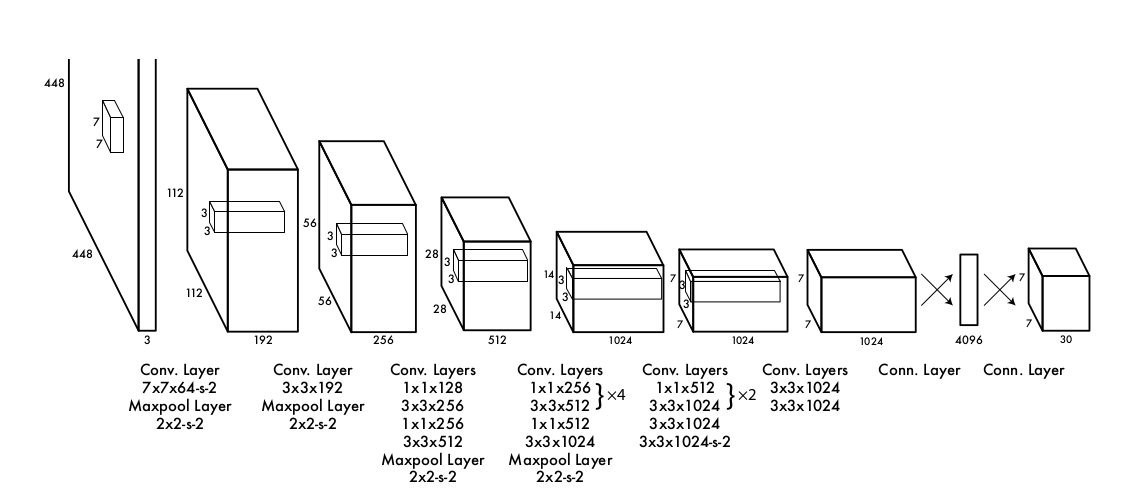
\includegraphics[scale=0.38]{Images/007_YOLO.png}
\caption{The YOLO Architecture[5]}
\label{The YOLO Architecture[5]}
\end{figure}

Diese Größe wird in diesem Projekt natürlich nicht erreicht, das Training würde viel zu lange dauern. Aber dieses Beispiel zeigt, wie Leistungsfähig Convolutional Networks im Bereich der Computer Vision sein können. 

Fangen wir nun mit dem ersten Kapitel an, in welchem wir uns die Fully Connected Layer ansehen werden.

\cleardoublepage
\section{Fully Connected Layer / Feed Forward Layer}
In diesem Kapitel werden die Fully Connected Layer betrachtet, welche genau so aufgebaut sind, wie bei den Feed Forward Networks. Genau genommen wird im Prinzip ein Feed Forward Network am Ende des Convolutional Networks eingesetzt, denn die Fully Connected Layer werden nur am Ende benutzt. Wenn in einem Netzwerk nur die Fully Connected Layer verwendet werden, handelt es sich um ein Feed Forward Network. 
Das Grundprinzip ist vergleichbar kompliziert. Jede Schicht enthält sogenannte Knoten. Diese Knoten sind mit den Neuronen in einem Gehirn vergleichbar.

\begin{figure}[H]
\centering
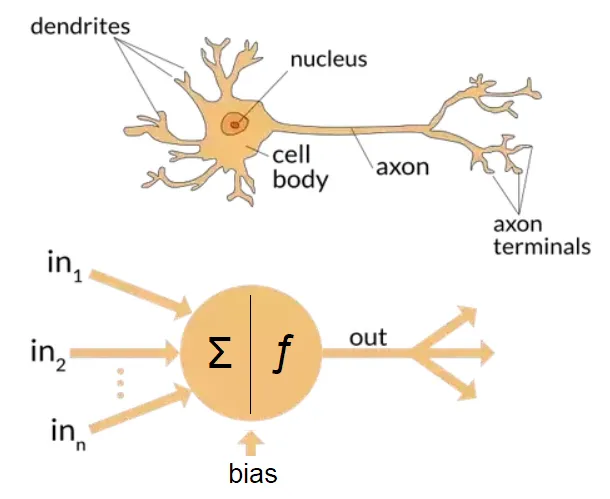
\includegraphics[scale=0.40]{./Images/001_DasNeuron.png}
\caption{Das Neuron}
\label{Das Neuron}
\end{figure}

Alle Knoten einer Schicht, sind mit allen Knoten der nächsten Schicht verbunden. Diese Verbindungen werden gewichtet, also müssen Gewichte gespeichert werden, die festlegen, wie wichtig der Input eines jeweiligen Knotens für den aktuellen Knoten ist. Diese Knoten können angepasst werden, das heißt, dass kleine inkrementelle Anpassungen mit jeder Lern-Iteration vorgenommen werden, um das Netzwerk Stück für Stück einem Fehler-Minimum anzupassen. 

\begin{figure}[H]
\centering
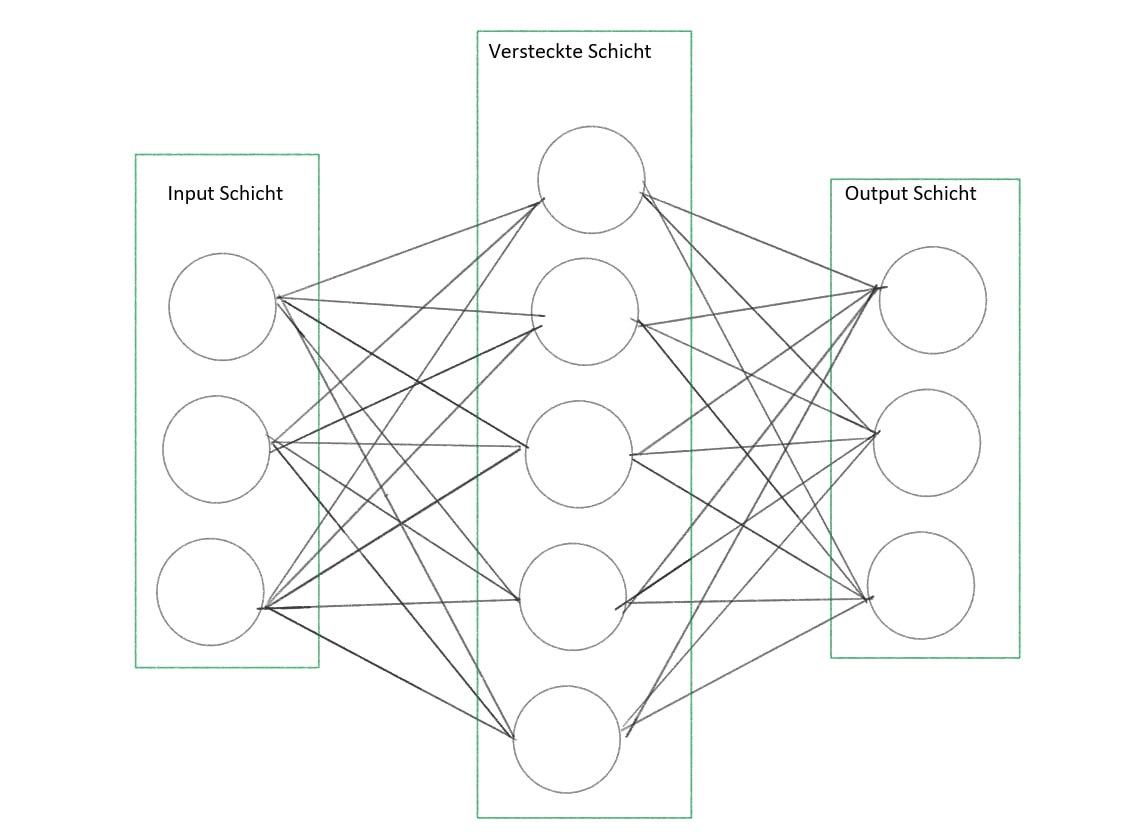
\includegraphics[scale=0.50]{./Images/002_FeedForwardNetzwerk.jpg}
\caption{Das Neuronale Netzwerk}
\label{Das Neuronale Netzwerk}
\end{figure}

Besonders für lineare Probleme, die nicht durch den Nullpunkt eines Koordinatensystems gehen ist es notwendig, auch Biases mit einzurechnen. Für die Bilderkennung ist das normalerweise nicht wichtig und da sich die Convolutions auf die Bilderkennung Spezialisieren, wird es für dieses Projekt nicht notwendig sein, Biases einzuplanen.

In diesem Kapitel werden nun zunächst der generelle Aufbau der Klasse "FullyConnectedLayer" dargelegt und in den beiden Unterkapiteln wird dann speziell auf den ForwardPass und auf die Backpropagation eingegangen, zusammen mit den mathematischen Grundlagen und dem dazugehörigen Code.

Zunächst muss die Klasse erstellt werden. Die Objektvariablen sind diese:
    
\begin{lstlisting}[language=Java]
public class FullyConnectedLayer extends Layer {
    double[][] weights;
    int inLength;
    int outLength;
    double learnRate;

    private double[] lastZ;
    private double[] lastInput;
\end{lstlisting} 
In den "weights" werden die Gewichte zwischen den Inputs und den Knoten der Schicht gespeichert. Diese können angepasst werden, um den Fehler des Netzwerkes zu minimieren und damit korrekte Klassifizierungen vornehmen zu können.
Mit "inLength" ist die Menge an Inputs gemeint, das heißt zum Beispiel wie viele Pixel die Bilder haben, die in die Schicht eingespeist werden.
Der Parameter "outLength" entspricht dann auch der Menge an Outputs welche von der Schicht erzeugt werden. Das hängt davon ab, wie viele Knoten die nächste Schicht hat, oder wenn es die letzte Schicht ist, wie viele mögliche Antworten das Netzwerk hat.
Die "learnRate" schränkt die Größe der Inkremente zwischen den einzelnen gelernten Bildern ein. Dies ist Notwendig, da die berechneten Inkremente, also die Steigung im Fehlergraphen, normalerweise zu groß sind und die Fehler Minima dadurch häufig übersprungen werden. Das Netzwerk soll sich aber dem Fehlerminimum langsam annähern, also müssen die Schritte kleiner sein. Zu klein sollten sie aber auch nicht sein, weil das Netzwerk dadurch deutlich langsamer wird und eine zu langsame Annäherung unter Umständen das Ziel nicht erreicht, bevor der Lernprozess abgeschlossen ist..


\begin{figure}[H]
\centering
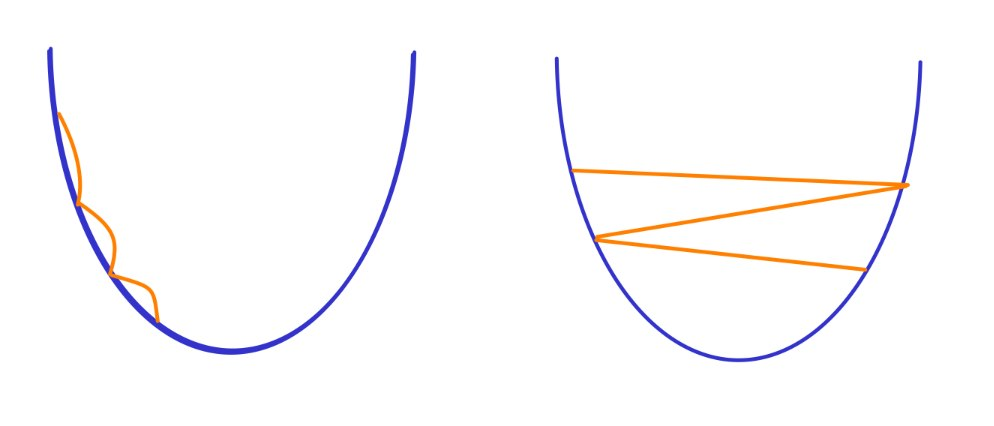
\includegraphics[scale=0.50]{./Images/006_LearnRate.jpg}
\caption{Learn Rate}
\label{Learn Rate}
\end{figure}

Mit dem Array "lastZ" und "lastInput" sollen jeweils für die Backpropagation notwendige Zwischenschritte gespeichert werden. "lastZ" entspricht den Inputs multipliziert mit den Gewichten. Das bedeutet: Hierbei handelt es sich um die Ergebnisse der Schicht bevor sie durch die Activation Funktion umgerechnet werden. Mit "lastInput" sind einfach die Inputs gemeint, die zuletzt in diese Schicht geleitet wurden und noch keinen Rechnungen unterlegen sind. Genaueres wird im Unterkapitel zur Backpropagation betrachtet, aber diese Werte werden uns später noch von Nutzen sein.


\subsection{Forward Propagation in der Fully Connected Layer}

Für den Forward Pass, also die Grundfunktion in der Query, muss ein Array erstellt werden, welches die Outputs der Schicht enthält. Beim Fully Connected Layer entspricht die Menge an Outputs der Menge der Knoten aus der nächsten Schicht. Ein Wert in der Outputmenge wird berechnet, indem jeder Input in die Schicht mit dem Gewicht multipliziert wird, welches zwischen jedem Knoten in dieser Schicht und dem Knoten der nächsten Schicht gespeichert wurde. Alle diese Werte werden dann multipliziert und mit einer Activation Funktion umgerechnet. Dies ist dann der Output, der an die nächste Schicht übergeben wird. Hier im Code wird dieser Output durch das Array "a" dargestellt, um auf das Ergebnis der Activation hinzuweisen.

Abgesehen davon werden allerdings auch noch die Werte lastInput und das Array "Z" zwischengespeichert. Diese Werte sind für die Backpropagation notwendig, daher werden die Details auch erst im nächsten Kapitel behandelt. Im Prinzip steht das Array "Z" für Zwischenergebnisse, die noch mit der Activation Funktion verrechnet werden müssen.

"lastInput" ist an sich selbsterklärend: Hier wird einfach der letzte Input zwischengespeichert, bevor diese weiter verrechnet werden.
\clearpage
\begin{lstlisting}[language=Java]
    public double[] FullyConnectedForwardPass(double[] input){
        lastInput = input;
        double[] Z = new double[outLength];
        double[] a = new double[outLength];
        //Diese schleife summiert alle Inputs auf alle outputs und multipliziert die Inputs mit ihren jeweiligen gewichten aus der weights-Matrix
        for(int i=0; i<inLength; i++){
            for(int j=0; j<outLength;j++){
                Z[j] += input[i]*weights[i][j];
            }
        }
        
\end{lstlisting}
Nach dieser Schleife sind die Inputs mit den Gewichten verrechnet, aber die Activation Funktion wurde noch nicht angewendet. Also sollten diese Werte unter "lastZ" zwischengespeichert werden.
\begin{lstlisting}[language=Java] 
        lastZ = Z;
		//Diese Schleife wendet auf alle Outputs die Activation Funktion an, in diesem Falle die Sigmoid Funktion
        for(int i=0; i<inLength; i++){
            for(int j=0; j<outLength;j++){
                a[j] = Sigmoid(Z[j]);
            }
        }
        return a;
    }
\end{lstlisting} 

Das Array welches zurückgegeben wird, ist der komplette berechnete Output und kann so an die nächste Schicht weitergeleitet werden. Im Convolutional Network kommen die Fully Connected Schichten immer ans Ende. Die Convolution Layer und die MaxPool Layer sind auf die Erkennung von Features in Bildern und auf die Komprimierung und Verdichtung relevanter Daten in den Bildern spezialisiert. Daher macht es keinen Sinn, diese Schichten nach einem Fully Connected Layer einzusetzen. Das Bild kann aus den Ausgaben einer Fully Connected Layer nicht wieder rekonstruiert werden und ist daher für die anderen Schichten nicht mehr nutzbar. Es kann also davon ausgegangen werden, dass nach einem Fully Connected Layer nur noch weitere Fully Connected Layer auftreten werden. 
Außerdem soll hier angemerkt werden, dass die Convolution und Pool Layer zwar die Bilderkennung positiv beeinflussen, simple Netzwerke bereits rein und ausschließlich mit Fully Connected Layern aufgebaut werden können. Diese sind zwar sehr anfällig für leichte Veränderungen der Inputs und die Genauigkeit kann geringer ausfallen, aber durchaus verlässliche Ergebnisse können damit schon erzielt werden.

Da die Outputs der Fully Connected Layer keine direkten Rückschlüsse auf die Bilder zulassen, die zu Anfang in das Netzwerk gegeben werden, wird bei den in der abstrakten Klasse definierten Methoden zur Rückgabe der verschiedenen Parameter auch anders verfahren, als in den anderen Layer-Klassen. Die anderen Layer-Klassen müssen Auskunft darüber geben können, wie viele Outputbilder sie erzeugen und welche Dimensionen diese besitzen. Zum Beispiel gibt die Max Pool Layer zwar komprimierte Bilder zurück, das heißt dass die Dimensionen kleiner geworden sind. Allerdings werden alle Bilder, die in die Schicht eintreten, mit jedem Filterfenster verrechnet, welches die Schicht besitzt. Das heißt die Menge der Outputbilder ist die Menge der Inputbilder mal die Menge der Filter. Diese Informationen sind für die nachfolgenden Schichten von großem Wert. Bei den Fully Connected Layern können nur Fully Connected Layer folgen, also ist auch nur die Menge der Inputs wichtig, da Fully Connected Layer die Inputs als ein einziges 1-Dimensionales Array betrachten. Also muss nur die "getOutputElements" Methode sinnvoll betrachtet werden, diese gibt einfach die "outLength" Variable zurück. Alle anderen get-Methoden können 0 zurück geben.

\begin{lstlisting}[language=Java] 
    public int getOutputElements() {
        return outLength;
    }
\end{lstlisting} 
\clearpage
\subsection{Backpropagation im Fully Connected Layer}
Backpropagation ist der Prozess, den Fehler, den ein Netzwerk macht zu quantifizieren und dann über alle Schichten zurückzuverfolgen. Dabei wird durch das Ableiten der Fehlerfunktion festgestellt, wie die Gewichte oder andere veränderbaren Attribute angepasst werden müssen, um sich dem Fehlerminimum zu nähern. Das Fehlerminimum wird durch kleine, inkrementelle Schritte angepeilt. Diese Schrittweise Annäherung nennt man Gradient Descent. 

Das Gradient Descent Verfahren funktioniert so, dass ein gegebenes Gewicht $w^0$ in die Fehlerfunktion $C_0$ eingesetzt wird, also die Funktion, die den Fehler quantifiziert, den das Netzwerk bei der Klassifizierung eines Bildes gemacht hat. Durch die Ableitung dieser Funktion an der gegebenen Stelle, kann eine Steigung berechnet werden, welche die Richtung angibt, in die das Gewicht angepasst werden sollte, um sich dem Fehlerminimum zu nähern. 
Das heißt also, wenn 

$C_0'(w^0)>0$, dann sollte das Gewicht $w^1$ ein Stück weiter links von $w^0$ sein und wenn

$C_0'(w^0)<0$, dann sollte das Gewicht $w^1$ ein Stück weiter rechts von $w^0$ sein.

Das lässt sich auch algorithmisch notieren:

$$w^k:=w^{k-1}-\lambda C'(w^{k-1}), k \geq 1$$

wobei $\lambda > 0$ ist, denn $\lambda$ entspricht der Learnrate, also dem Skalierungsmaß für die Inkremente, in denen die Gewichte angepasst werden. Ohne das Skalierungsmaß wären die Anpassungen zu groß und würden die Fehlertiefpunkte regelmäßig weit überspringen, anstatt sich ihnen anzunähern [1, S.114 ff.]. 

Zuerst sollte man die Fehlerfunktion betrachten. 
Es sei der letzte Output aus dem Netzwerk genannt $O_L$. Außerdem werden die Targets, also die angestrebten Werte, für das Bild benötigt. Um ein Neuronales Netzwerk zu trainieren, braucht man nicht nur die zu klassifizierenden Inputs, diese Inputs müssen auch mit Labeln versehen sein. Ein Label gibt an, was auf dem Bild zu sehen ist. Das Ziel ist es, dass das Netzwerk eine Ausgabe macht, die sich möglichst wenig von dem Label unterscheidet. Hier kommen die Targets zum tragen. Im Prinzip erstellt man ein Array, welches für jede Antwortmöglichkeit des Netzwerkes ein Feld besitzt. Das Feld, das dem Label entspricht, wird auf 1 gesetzt, alle anderen Felder werden auf 0 gesetzt. Dies sind die Targets $T$.

Um nun die Loss oder auch Cost Funktion $C$, also die Fehlerfunktion zu berechnen, müsste man nur die Targets von den Outputs abziehen, allerdings sollten die Ergebnisse noch Quadriert werden. Das hat zwei Vorteile, der erste Vorteil ist, dass Fehler dadurch betont werden. Große Fehler haben dadurch einen noch größeren Einfluss. Das hilft, sich nicht zu schnell oder zu langsam dem Fehlerminimum anzupassen. Der zweite Vorteil ist, dass durch das Quadrieren alle Fehler positiv werden. Alle Fehler müssen nachher summiert werden. Wenn es positive und negative Fehler gibt, würden sich diese gegenseitig aufheben. 
Alles in allem sieht die Fehlerfunktion für dieses Netzwerk dann so aus:

$$C_0 = (O_L - T)^2$$

Nun gilt es, herauszufinden, wie sich die Fehlerfunktion ändert, im Bezug auf die Gewichte und anderen veränderbaren Parameter im Netzwerk.

Dazu kann man notieren, dass die Ableitung von $C_0$ gesucht ist, im Bezug auf eine Änderung an $w_L$, damit gemeint sind die Gewichte aus der letzten Schicht.

$$\frac{\delta C_0}{\delta w_L}$$

Diese Ableitung lässt sich dank der Kettenregel weiter aufschlüsseln, sodass einzelne Komponenten entstehen, die mit Code berechnet werden können.

$$\frac{\delta C_0}{\delta w_L}=
\frac{\delta Z_L}{\delta w_L}*
\frac{\delta a_L}{\delta Z_L}*
\frac{\delta C_0}{\delta a_L}$$

Diese Terme können einzeln entschlüsselt und im Code verwendet werden. Der erste Term ist

$$\frac{\delta Z_L}{\delta w_L}$$

und beschreibt die Ableitung der Berechnung in den Knoten bevor die Transferfunktion, also zum Beispiel die Sigmoid Funktion eingesetzt wird, im Bezug zu den Gewichten der letzten Schicht.
Diese Berechnung sieht erst einmal so aus:

Jede Schicht besitzt eine Menge an Knoten, die den Neuronen des Gehirns nachempfunden sind. Ein Knoten ist mit allen Inputs verknüpft, also mit dem Bild das in die erste Schicht geleitet wird, oder alle Ausgaben der vorigen Schicht, wenn es sich nicht um die erste Schicht handelt. Diese Verbindungen sind gewichtet, um die Stärke der synaptischen Verknüpfung zwischen den Neuronen darzustellen. Diese Gewichte werden bei der Backpropagation angepasst. Im Netzwerk werden die Gewichte in einer Matrix gespeichert, hier heißt sie "weights". 

Um einen einzelnen Knoten k zu berechnen iteriert man über alle Inputs, multipliziert diese mit dem jeweiligen Gewicht zwischen dem Input und dem Knoten, also $w_{ik}$ und summiert die Ergebnisse:


$$Z_{Lk}=\sum_{i = 1}^{n}w_{ik}*x_i$$

Im Prinzip muss also nur der Term $w_{ik}*x_i$ im Bezug auf die Gewichte abgeleitet werden, um die Änderungsrate berechnen zu können, wenn die Gewichte angepasst werden.

$$\frac{\delta Z_L}{\delta w_L}=x_i$$

Wie wir sehen entspricht x einfach den Inputs aus der vorigen Schicht. Diese sollten also beim Forwardpass auf jeden Fall immer zwischengespeichert werden, um hier in der Backpropagagtion benutzt werden zu können. Dies wurde im letzten Kapitel schon vorbereitet.

Der nächste Term 
$$\frac{\delta a_L}{\delta Z_L}$$ Beschäftigt sich mit dem Einfluss von $Z_L$ auf die Ableitung von der Activation Funktion. Es gibt verschiedene Transferfunktionen $T(x)$ und zwei werden besonders häufig verwendet. Zum einen die Sigmoid Funktion, zum anderen ReLu. 
ReLu ist besonders leicht zu berechnen und wird daher für schnelleres Lernen eingesetzt. Alle Werte unter 0 werden zu 0 Transformiert und ausgegeben, alle Werte über 0 werden so zurückgegeben, wie sie sind.

$$
T(x):=
\left\{
\begin{tabular}{l}
0 für $x<0$ \\
x für $x\geq 0$
\end{tabular}
\right\}
:=T_1(x)
$$

Die Ableitung davon ist auch denkbar einfach, Unter 0 hat die x keinen Einfluss, über 0 hat es einen direkten Einfluss, also 1.

$$
T'(x):=
\left\{
\begin{tabular}{l}
0 für $x<0$ \\
1 für $x\geq 0$
\end{tabular}
\right\}
:=T'_1(x)
$$

Etwas aufwändiger ist die Sigmoid Funktion, die auch in diesem Netzwerk verwendet werden soll. Die Sigmoid Funktion sieht so aus:

$$\sigma (x)=\frac{1}{(1+e^{-x})}$$
Und ihre Ableitung:
$$\sigma '(x)=\sigma (x)(1-\sigma(x))$$

%TODO Es kann hier noch die Ableitung der Sigmoid erklärt werden, so wie Prof Lanz sich das gewünscht hat. Allerdings ist dies Extrem aufwändig und nicht zu empfehlen...

Hier ist der Code für die Sigmoid Funktion und ihre Ableitung:
\begin{lstlisting}[language=Java] 
    //Die Sigmoid Funktion
    public double Sigmoid(double weightedInput) {
        return 1.0 / (1 + Math.exp(-weightedInput));
    }
    //Die Ableitung der Sigmoid Funktion
    public double SigmoidAbleitung(double weightedInput) {
        double activation = Sigmoid(weightedInput);
        return activation * (1.0 - activation);
    }
    
\end{lstlisting} 

Und hier ist die Relu Funktion mit ihrer Ableitung. Im Code sehr einfach umzusetzen:

\begin{lstlisting}[language=Java] 
    //Die ReLu Funktion
    public double ReLu(double weightedInput) {
        if (weightedInput <= 0)
        return 0.0;
    else
        return weightedInput;
    }
        
    //Die Ableitung der ReLu Funktion
    public double ReLuAbleitung(double weightedInput) {
        if (weightedInput <= 0)
            return 0.01; //Leak Value, um Tote bereiche zu vermeiden. Vermutlich bei Sigmoid kein Problem
        else
            return 1.0;
    }
\end{lstlisting} 

Nun kommen wir zum vorerst letzten Term:

$$\frac{\delta C_0}{\delta a_L}$$

Gesucht wird die Ableitung der Cost oder Fehlerfunktion, im Bezug auf die Outputs der letzten Schicht im Netzwerk. Dies ist die Fehlerfunktion:

$$C_0 = (O_L - T)^2$$

Hierbei ist $O_L$ gleich $a_L$ des Netzwerkes.
Die Ableitung hier ist einfach:

$$\frac{\delta C_0}{\delta O_L} = 2(O_L - T)$$

Damit sind alle Terme der letzten Schicht im Netzwerk geklärt und können eingesetzt werden.
Um im Code nachvollziehen zu können, welcher Wert was macht, nennen wir die Werte einfach genau so, wie sie geschrieben werden.


$$\frac{\delta Z_L}{\delta w_L} \rightarrow dZdw $$ \\
$$\frac{\delta a_L}{\delta Z_L} \rightarrow dadZ $$ \\
$$\frac{\delta C_0}{\delta a_L} \rightarrow dCda $$ \\

Nachdem die Namenskonvention geklärt ist, kann der Code erstellt werden:

\begin{lstlisting}[language=Java] 
    public void backPropagation2(double[] dCda) {
        double dZdw;
        double dadZ;
        double dCdw;

        for(int k=0; k<inLength; k++){
            for(int j=0; j<outLength; j++){
                dZdw = lastInput[k];
                dadZ = SigmoidAbleitung(lastZ[j]);

                dCdw = dZdw * dadZ * dCda[j];

                weights[k][j] -= dCdw*learnRate;
            }
        }
    }
\end{lstlisting} 

Um die Methode Modular zu halten, wird die Ableitung vom Error außerhalb der Methode berechnet und als "dCda", also Ableitung der Cost Funktion im Bezug auf die Outputs der letzten Schicht, an die Methode übergeben. Dadurch wird die Backpropagation angestoßen. Als nächstes werden die Variablen aufgestellt. Das Ziel ist es, "dCdw", also die Cost Funktion im Bezug auf die Gewichte zu ermitteln. 
In einer verschachtelten Schleife über alle Gewichte werden die Variablen zunächst belegt.
Warum über alle Gewichte? Weil die Änderung für jedes Gewicht berechnet werden soll. 
"dZdw" Entspricht dem letzten Input aus der vorletzten Schicht. "dadZ" ist das Ergebnis der Ableitung der Transferfunktion, hier Sigmoid, im Bezug auf die gewichteten Inputs der vorletzten Schicht.
Um also das Ergebnis der Ableitung der Cost Funktion im Bezug auf die Gewichte der letzten Schicht im Netzwerk zu berechnen, müssen diese Zwischenergebnisse nur noch multipliziert werden. Das heißt die entsprechenden Werte von "dCda", die übergeben wurden, multipliziert mit "dZdw" und "dadZ".
Das Ergebnis dieser Rechnung ist die Steigung der Fehlerfunktion, an der Stelle, an der das jeweilige Gewicht eingesetzt wurde. Wenn die Steigung positiv ist, sollte das Gewicht verringert werden, also abgezogen werden, um sich dem Fehlerminimum anzunähern.
Wenn die Steigung negativ ist, liegt das Fehlerminimum voraus, also sollte das Gewicht vergrößert werden.
Wichtig an dieser Stelle ist noch zu beachten, dass die berechnete Änderungsrate zu groß ist und mit der LearnRate multipliziert werden muss, bevor der Wert von den Gewichten abgezogen wird. Es könnte sonst dazu kommen, dass das Fehlerminimum übersprungen wird.

Dies ist die vollständige Berechnung der Anpassung der Gewichte in der letzten Schicht. Aber nun stellt sich die Frage: Wie wird die vorletzte Schicht angepasst? und die Schicht davor?

Im Prinzip muss der Fehler weiter durch das Netzwerk zurückgereicht werden und in jeder Schicht, die anpassbare Parameter hat, müssen diese Parameter so angepasst werden, wie sie für den Fehler verantwortlich waren.

Dies kann vollständig modular aufgebaut werden, sodass eine völlig variable Anzahl an Schichten möglich werden. Wenn man die Ableitung der Cost Funktion im Bezug auf die Gewichte der letzten Schicht und die Ableitung der Cost Funktion im Bezug auf die Gewichte der vorletzten Schicht miteinander vergleicht, so fällt auf, dass es Terme gibt, die zum Teil völlig gleich sind, dass es einen Term gibt der sich verändert und dass es zwei neue Terme gibt, die sich von alten Termen nur darin unterscheiden, dass sie Inputs aus der Vorletzten, anstatt aus der letzten Schicht benötigen.

Diesmal wird die Änderungsrate der Cost Funktion $C$ gesucht, in Abhängigkeit von den Gewichten der vorletzten Schicht, $w_{(L-1)}$.

$$\frac{\delta C_0}{\delta w_{(L-1)}}=
\frac{\delta Z_{(L-1)}}{\delta w_{(L-1)}}*
\frac{\delta a_{(L-1)}}{\delta Z_{(L-1)}}*
\frac{\delta Z_L}{\delta a_{(L-1)}}*
\frac{\delta a_L}{\delta Z_L}*
\frac{\delta C_0}{\delta a_L}*
$$

Die letzten beiden Terme sind schon aus der vorherigen Rechnung bekannt.

$$\frac{\delta a_L}{\delta Z_L}$$
$$\frac{\delta C_0}{\delta a_L}$$

Damit gemeint sind die Ableitung der Cost Funktion, sowie die Ableitung der Activation Funktion. Diese können bereits in der letzten Schicht verrechnet werden und an die vorletzte Schicht übergeben werden. Außerdem kann die Ableitung des dritten Terms ebenfalls in der letzten Schicht berechnet und übergeben werden. Dieser Unterscheidet sich von dem dritten Term in den Berechnungen für die letzte Schicht. Anstatt die Änderungsrate im Bezug auf Änderungen an den Gewichten, berechnet dieser Term die Änderungsraten im Bezug auf die Änderungen an den Inputs aus der vorherigen Schicht.

$$\frac{\delta Z_L}{\delta a_{(L-1)}}$$

Die Ableitung der Berechnung der Gewichteten Outputs der letzten Schicht, im Bezug auf die Inputs der vorletzten Schicht. Die Änderungsrate hängt hierbei völlig von den Gewichten der letzten Schicht ab, also gilt:

$$\frac{\delta Z_L}{\delta a_{(L-1)}} = w_L$$

Wenn diese drei Terme bereits in der letzten Schicht berechnet werden, können sie ohne weiteres an die vorletzte Schicht übergeben werden. Nach diesem Prinzip können beliebig viele Schichten aneinander gereiht werden und sich gegenseitig ihre berechneten Werte durchreichen. 

Die bisherigen Werte kann man zusammenfassen:

$$
\frac{\delta Z_L}{\delta a_{(L-1)}}*
\frac{\delta a_L}{\delta Z_L}*
\frac{\delta C_0}{\delta a_L}
= \frac{\delta C_0}{\delta a_{(L-1)}}
$$

$\frac{\delta C_0}{\delta a_{(L-1)}}$ kann einfach an die nächste Backpropagation Methode übergeben werden.

Dort, in der vorletzten Schicht, wird das gleiche getan, wie zuvor in der letzten Schicht. Die Eingabe, "dCda", wird mit diesen Termen verrechnet:

$$
\frac{\delta Z_{(L-1)}}{\delta w_{(L-1)}}*
\frac{\delta a_{(L-1)}}{\delta Z_{(L-1)}}*
\frac{\delta C_0}{\delta a_{(L-1)}}
$$

Diese Terme sind im Prinzip die gleichen wie zuvor, nur auf die aktuelle Schicht gemünzt. 

Um eine kleine Zusammenfassung zu schaffen:

Jede Schicht muss 3 Terme miteinander multiplizieren. 

Der erste Term beschreibt die Ableitung der Cost Funktion im Bezug auf die Outputs der aktuellen Schicht. Bei der letzten Schicht im Netzwerk, also der ersten Schicht im Backpropagationverfahren, ist das einfach die Ableitung der Cost Funktion, welche zum Berechnen die Outputs des Netzwerks und die erwarteten Werte der Inputs des Netzwerkes benötigt. In allen weiteren Schichten handelt es sich dabei um errechnete Werte aus den anderen Schichten, welche übergeben werden. Ab hier werden sie im Code "dCd0" genannt, da der Name "dZda" anderweitig noch gebraucht wird.

Der zweite Term sieht in jeder Schicht gleich aus, es kommt hierbei lediglich auf die Inputs an. Es handelt sich um die Ableitung der Activation Funktion, im Bezug auf die gewichteten Inputs.

$$\frac{\delta a}{\delta Z}$$

Dieser Schritt wurde zuvor schon implementiert.
Übrig bleibt also nur der letzte Term. diesen gibt es in zwei Ausführungen und zwar einmal um die Gewichte der aktuellen Schicht anzupassen und einmal um die Werte zu berechnen, die an die nächste Schicht im Backpropagationverfahren gereicht werden sollen.
Um die Gewichte anzupassen, benötigt man hierbei die Inputs aus der letzten Schicht und auch dies wurde bereits implementiert. Es bleibt nur noch die Berechnung für die nächste Schicht. Wie weiter oben schon festgestellt, handelt es sich dabei um die Gewichte der aktuellen Schicht. 
Nun zur Form: Es geht immer noch darum, die Fehler, die das Netzwerk gemacht hat, an die Schichten weiterzureichen. Daher muss ein Vektor erstellt werden, der den Outputs der vorherigen Schicht entspricht und die Fehler enthält, die von der Schicht verursacht wurden.
Dieser Vektor wird nun "dCda" genannt, denn er soll immerhin die Änderungsraten enthalten, die durch die Ableitung der Cost Funktion im Bezug auf die Outputs "$a$" der vorherigen Schicht berechnet wurden. Eine weitere neue Variable ist der double "dZda", welcher schlichtweg das Gewicht enthält, welches gerade angepasst werden soll.

\begin{lstlisting}[language=Java]
    public void backPropagation(double[] dCd0) {
        double[] dCda = new double[inLength];
        double dZdw;
        double dadZ;
        double dCdw;
        double dZda;
\end{lstlisting} 
In der äußeren Schleife wird nun eine Variable "dCda\_sum" geführt. In dieser werden alle Änderungsraten der Cost Funktion im Bezug auf die Inputs der letzten Schicht aufsummiert. Dieser Wert wird für jeden Input der aktuellen Schicht erstellt und im Vektor "dCda" gespeichert.
\begin{lstlisting}[language=Java]  
        for(int k=0; k<inLength; k++){
            double dCda_sum = 0;

            for(int j=0; j<outLength; j++){
                dZdw = lastInput[k];
                dadZ = SigmoidAbleitung(lastZ[j]);
\end{lstlisting} 
In der inneren Schleife werden nun auch die entsprechenden Gewichte festgehalten. Wie zuvor werden nun die Änderungsraten für die aktuellen Gewichte berechnet und angewandt.
\begin{lstlisting}[language=Java]  
                dZda = weights[k][j]; 
                dCdw = dZdw * dadZ * dCd0[j];
                weights[k][j] -= dCdw*learnRate;
\end{lstlisting} 
Zuletzt wird aber die Änderungsrate der Cost Funktion im Bezug auf die Inputs der vorherigen Schicht berechnet. Statt dem letzten Input wird hier das aktuelle Gewicht multipliziert und zur variable "dCda\_sum" hinzugefügt.
\begin{lstlisting}[language=Java]              
                dCda_sum += dZda * dadZ * dCd0[j];
            }
            dCda[k] = dCda_sum;
        }
\end{lstlisting} 
Nach den Schleifen muss nur noch die Backpropagation Methode der vorherige Schicht aufgerufen werden und dieser der Vector "dCda" übergeben werden.
\begin{lstlisting}[language=Java]   
        if(previousLayer!= null){
            previousLayer.backPropagation(dCda);
        }
    }
\end{lstlisting} 

Dieser Prozess muss zwar noch in den anderen Layern implementiert werden, aber auf diese elegante Weise kann die Backpropagation Methode umgesetzt werden. Wenn man das Netzwerk ausschließlich aus Fully Connected Layern aufbaut, funktionieren klassifikatorische Aufgaben schon ganz gut. Durch den Einsatz von Pooling Layern und Convolutional Layern sollte die Effizienz allerdings noch weiter gesteigert werden können.

\cleardoublepage
\section{Pooling Layer}
Pooling Layer werden dazu verwendet, um das sogenannte Downsampling zu betreiben. Downsampling bedeutet einfach, dass eine geringere Auswahl an Daten weitergegeben werden.
In einem Netzwerk benutzt man eines dieser Verfahren, um die weiteren Schichten nur mit den nötigsten Daten zu belasten. Gerade in Anbetracht der Größe der Daten, die bei den Convolutional Layern entstehen, kann das viel Zeit sparen. Hauptsächlich sorgt dies auch dafür, dass das Netzwerk weniger anfällig für Veränderungen der Daten wird. Leichte Veränderungen der Daten können für gravierende Änderungen sorgen, das heißt wenn ein Bild nicht korrekt zentriert ist, oder wenn es um ein paar Grad gedreht wird, kommt ein Netzwerk schnell durcheinander.
Die Convolution Layer erstellen Feature Maps, in denen die Features allerdings auch die gleichen Positionen haben, wie in den Inputs. Dadurch können bei kleinen Veränderungen schon Fehler in den nächsten Schichten entstehen. Dem kann man durch das Downsampling entgegenwirken.

Auf eine gewisse Weise können die Daten bereits in den Convolutional Layern "gedownsampelt" werden, wenn die Schrittgröße (Stride) beim Anwenden der Filter größer ist als 1.

Nun stellt sich die Frage: Wie genau funktioniert ein Pooling Layer dann? So wie bei den Convolutional Layern werden Filter eingesetzt. Diese sind aber kleiner und funktionieren anders. Meist ist ein Filter hier nur 2x2 groß und bei der Anwendung wird eine Schrittgröße von 2 verwendet. Die Filter überlappen die Felder nicht, die bereits behandelt wurden. 
Auf die Pixel, auf die der Filter angewandt wird, wird nun eine Pooling Operation durchgeführt. 

Zwei mögliche Pooling Operationen sind das Average Pooling und das Maximum Pooling. 
\begin{itemize}
  \item Das Average Pooling gibt den Durchschnitt aller Werte als Output zurück, während
  \item das Maximum Pooling nur den größten Wert der betrachteten Werte zurückgibt.
\end{itemize}
Es gibt noch weitere, wie zum Beispiel das Globale Pooling, bei dem die gesamte Feature Map auf einen einzigen Wert reduziert wird. Dadurch soll auf eine möglichst aggressive Art festgestellt werden, ob ein bestimmtes Feature überhaupt in der Feature Map vorkommt. Je nach Anwendungsfall kann auch diese Methode Erfolg bringen.

Zunächst wird die Maximum Pooling Layer betrachtet.
genau wie bei den Convolutional Layern, wird hier eine StepSize verwendet. Zwar ändert sich diese in den meisten Fällen nicht, aber es ist gut, die Flexibilität zu haben.
Die windowSize legt fest, welche Dimensionen der Filter haben soll.
\\Außerdem ist es hilfreich, wenn die Inputparameter auch gespeichert werden. Damit gemeint sind input length, input rows und input columns, also die Menge an Bildern, zusammen mit den Zeilen und Reihen die diese Bilder haben.

\begin{lstlisting}[language=Java]
public class MaxPoolLayer extends Layer {

    private int stepSize;
    private int windowSize;

    private int inLength;
    private int inRows;
    private int inCols;
\end{lstlisting} 

\subsection{Forward Propagation im Pooling Layer}
Wie oben beschrieben, wird hier ein kleiner Filter benutzt, der über die Inputbilder gleitet und entweder den maximalen Wert, oder den Durchschnittswert zurückgibt. 

\begin{figure}[H]
\centering
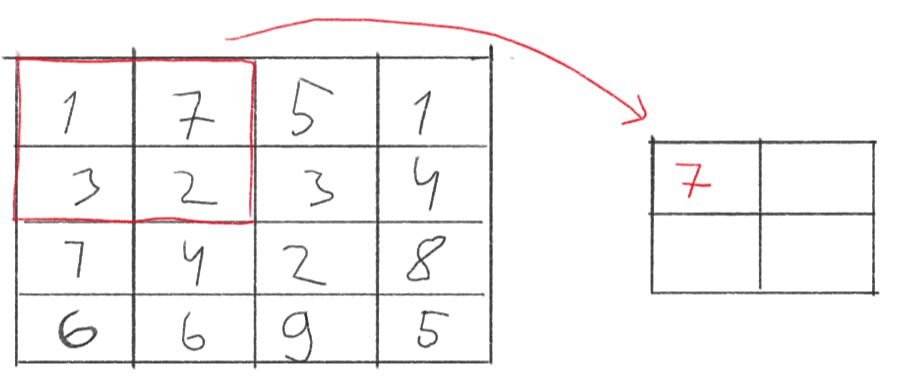
\includegraphics[scale=0.40]{Images/008_MaxPool1.jpg}
\caption{Max Pool Schritt  1}
\label{Max Pool Schritt  1}
\end{figure}

\begin{figure}[H]
\centering
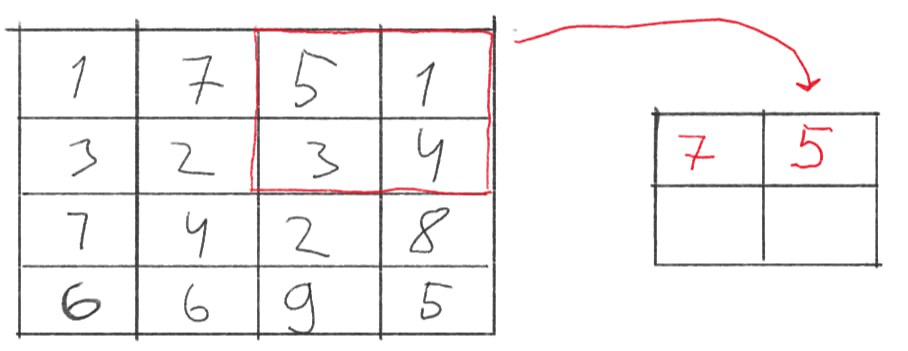
\includegraphics[scale=0.40]{Images/009_MaxPool2.jpg}
\caption{Max Pool Schritt 2}
\label{Max Pool Schritt  2}
\end{figure}

Zunächst wird eine Methode benötigt, die den Filter darstellt und eine Feature Map durchläuft. 

\begin{lstlisting}[language=Java]
 public double[][] pool(double[][] input){
 		//Die Output Dimensionen müssen berechnet werden
        double[][] output = new double[getOutputRows()][getOutputCols()];
        //zwei Schleifen um über den Input zu Iterieren
        for(int r=0; r<getOutputRows(); r+=stepSize){
            for(int c=0; c<getOutputCols(); c+=stepSize){
                double max = 0.0;
                //Zwei Schleifen um das Maximum im Fenster des Filters zu finden
                for(int x=0; x<windowSize; x++){
                    for(int y=0; y<windowSize; y++){
                        if(max<input[r+x][c+y]){
                            max=input[r+x][c+y];
                        }
                    }
                }
                output[r][c] = max;
            }
        }
        return output;
    }
\end{lstlisting}
Alternativ kann natürlich auch der Durchschnitt errechnet und ausgegeben werden. Dazu sind keine großen Anpassungen nötig:
\begin{lstlisting}[language=Java]
 public double[][] pool(double[][] input){
 		//Die Output Dimensionen müssen berechnet werden
        double[][] output = new double[getOutputRows()][getOutputCols()];
        //zwei Schleifen um über den Input zu Iterieren
        for(int r=0; r<getOutputRows(); r+=stepSize){
            for(int c=0; c<getOutputCols(); c+=stepSize){
                double average = 0.0;
                //Zwei Schleifen um die Werte im Fenster des Filters zu addieren
                for(int x=0; x<windowSize; x++){
                    for(int y=0; y<windowSize; y++){
                    	average+=input[r+x][c+y];
                    }
                }
                //Der Durchschnitt muss natürlich noch durch die Menge der im Filterfenster enthaltenen Pixel geteilt werden
                output[r][c] = average/(windowSize*windowSize);
            }
        }
        return output;
    }
\end{lstlisting}
Im Code wurden die Methoden getOutputRows und getOutputCols schon verwendet, also müssen diese auch noch implementiert werden. Die Formel dazu sieht folgendermaßen [2] aus:
$$H_{out} = floor(1 + (H - pool\_height)/stride)$$
$$W_{out} = floor(1 + (W - pool\_ width)/stride)$$

$H_{out}$ und $W_{out}$ entsprechen den Dimensionen des output Fensters. 

Und im Code werden diese so umgesetzt:

\begin{lstlisting}[language=Java]
    public int getOutputRows() {
        return (inRows - windowSize) / stepSize + 1;
    }

    public int getOutputCols() {
        return (inCols - windowSize) / stepSize + 1;
    }
\end{lstlisting}

\subsection{Backpropagation im Pooling Layer}
Für die Backpropagation in einem Pooling Layer müssen keine Gewichte oder Biases angepasst werden. Denn diese gibt es hier nicht. Stattdessen muss der Fehler aber trotzdem auf einen der Inputs zurückgeführt werden, das heißt zum Beispiel, dass beim Max Pooling aus jedem von dem Filterfenster betrachteten Gebiet der maximale Wert für den Fehler verantwortlich war und die anderen Werte keine Verantwortung tragen. 

%TODO Bild einfügen

Am besten gelingt dies, indem die Positionen der maximal Werte gespeichert werden.
Dazu sollten erst neuen Instanzvariablen angelegt werden:


\begin{lstlisting}[language=Java]
    List<int[][]> lastMaxRow;
    List<int[][]> lastMaxCol; 
\end{lstlisting}

Wir erstellen zwei Listen, welche 2-Dimensionale Arrays enthalten. Jeweils eine Liste für die Koordinate der X und eine für die Y Achse.
Danach müssen diese initialisiert werden und zwar in der "maxPoolForwardPass" Methode. Das stellt sicher, dass sie initialisiert werden, bevor das pooling beginnt:

\begin{lstlisting}[language=Java]
    public List<double[][]> maxPoolForwardPass(List<double[][]> input) {
        //Initialisierung der lastMaxRow und Col, in denen die Position der Maximalen Werte gespeichert werden
        lastMaxRow = new ArrayList<>();
        lastMaxCol = new ArrayList<>();
\end{lstlisting}

Um die Werte dann zu speichern, müssen diese während der pooling Operation gespeichert werden.
Dazu können zwei 2-Dimensionale Integer Arrays verwendet werden, welche mit den gleichen Maßen initialisiert werden, wie die Outputs. Das heißt, dass für jeden Output die X und Y Koordinate im dazugehörigen lastMax-Array ein entsprechender Platz vorhanden ist.

\begin{lstlisting}[language=Java]
public double[][] pool(double[][] input) {
        double[][] output = new double[getOutputRows()][getOutputCols()];

        int[][] maxRows = new int[getOutputRows()][getOutputCols()];
        int[][] maxCols = new int[getOutputRows()][getOutputCols()];   
\end{lstlisting}
Für den Fall, das kein maximum über 0 gefunden werden konnte, sollten Koordinaten trotzdem markiert werden, darum werden die alle Felder zuerst auf -1 gesetzt:
\begin{lstlisting}[language=Java]
        for (int r = 0; r < getOutputRows(); r += stepSize) {
            for (int c = 0; c < getOutputCols(); c += stepSize) {
                double max = 0.0;

                maxRows[r][c] = -1;
                maxCols[r][c] = -1;
\end{lstlisting}
In der inneren Schleife müssen die Koordinaten natürlich auch gespeichert werden, wenn ein neues Maximum im Fenster gefunden wurde:
\begin{lstlisting}[language=Java]
                for (int x = 0; x < windowSize; x++) {
                    for (int y = 0; y < windowSize; y++) {
                        if (max < input[r + x][c + y]) {
                            max = input[r + x][c + y];
//Koordinaten des Maximalen Wertes werden in den dafür vorgesehenen Arrays gespeichert
                            maxRows[r][c] = r + x;
                            maxCols[r][c] = c + y;
                        }
                    }
                }
                output[r][c] = max;
            }
        }
\end{lstlisting}
Zuletzt müssen die Arrays, welche die Koordinaten enthalten noch den Listen hinzugefügt werden, die am Anfang initialisiert wurden:
\begin{lstlisting}[language=Java]
        lastMaxRow.add(maxRows);
        lastMaxCol.add(maxCols);
        return output;
    }
\end{lstlisting}

Die eigentliche Umsetzung der Backpropagation findet in der "backPropagation" Methode statt. Der Grundgedanke ist, dass nur der Maximalwert zum Fehler beigetragen hat und daher auch nur dieser Wert angepasst werden muss. Also erstellt man eine Fehlermatrix, die überall nur 0 enthält, außer an den Stellen, von denen die Maximalwerte genommen wurden. Dort werden die Fehlerwerte eingetragen und dann, da es hier keinerlei Gewichte oder Biases gibt, wird diese Fehlermatrix an die nächste Schicht weitergegeben.
Zuerst muss eine Liste mit den Fehlermatrizen erstellt und initialisiert werden. Es wird ein Zähler benötigt, um über alle vorher angelegten Koordinaten-Matrizen zu iterieren, welche die Positionen der Maximalwerte enthalten.
\begin{lstlisting}[language=Java]
    public void backPropagation(List<double[][]> dLdO) {
        List<double[][]> dXdL = new ArrayList<>();
        int l=0;
\end{lstlisting}
Dann wird über alle eingehenden Fehlermatrizen iteriert, um die jeweilige Fehlermatrix zu erstellen, die an die nächste Schicht weitergegeben wird. Letztere muss zunächst initialisiert werden.  
\begin{lstlisting}[language=Java]
        for(double[][] array : dLdO){
            double[][] error = new double[inRows][inCols];
\end{lstlisting}
Dann muss die eingehende Fehlermatrix durch iteriert werden. Für jeden eingehenden Wert wird die Position des verantwortlichen Maximalwerts ermittelt. In der entstehenden Fehlermatrix wird der eingehende Fehler dann an der jeweiligen Position hinzugefügt. Wichtig ist, dass der Wert zu den bestehenden Werten hinzugefügt wird. 
Meistens überlappen sich die betrachteten Fenster in der Pooling Phase nicht, aber falls doch, kann ein Wert in mehreren Fenstern der Maximalwert sein. 
Daher ist dieser Wert dann auch für mehrere Fehler verantwortlich. Das wird dadurch ausgedrückt, das der Fehlerwert dann aufaddiert wird.
\begin{lstlisting}[language=Java]
            for(int r=0; r<getOutputRows(); r++){
                for(int c=0; c<getOutputCols(); c++){
                    int max_i = lastMaxRow.get(l)[r][c];
                    int max_j = lastMaxCol.get(l)[r][c];

                    if(max_i != -1){
                        error[max_i][max_j] += array[r][c];
                    }
                }
            }
\end{lstlisting}
Zuletzt müssen die entstandenen Fehlermatrizen nur noch der Liste hinzugefügt werden, welche dann an die nächste Schicht weitergegeben wird.  
\begin{lstlisting}[language=Java]
            dXdL.add(error);
            l++;
        }
        if(previousLayer != null){
            previousLayer.backPropagation(dXdL);
        }
    }
\end{lstlisting}

Für den Fall, dass die eingehenden Fehler keine Liste, sondern ein einfaches Array ist, also zum Beispiel weil die nächste Schicht eine Fully Connected Layer ist, erstellt man noch eine "backPropagation" Methode:

\begin{lstlisting}[language=Java]
    public void backPropagation(double[] dLdO) {
        List<double[][]> matrixList = vectorToMatrix(dLdO, getOutputLength(), getOutputRows(), getOutputCols());
        backPropagation(matrixList);
    }
\end{lstlisting}
Diese Methode wandelt zuerst das Array in eine Matrix um und übergibt diese dann an die erste "backPropagation" Methode. Die Umwandlung benötigt natürlich auch bestimmte Parameter, um das Array richtig umzuwandeln. Die Werte müssen im gleichen Format vorliegen, wie die Ausgabewerte dieser Schicht, daher benötigen wir die Angaben zu der Ausgabemenge und den Zeilen und Spalten der Feature Map.

\cleardoublepage
\section{Convolutional Layer}
Dieses Kapitel beschäftigt sich mit dem Namensgeber des gesamten Netzwerks: Das convolutional Layer. 
In dieser Schicht geht es darum, bestimmte Features zu erkennen und diese in einer sogenannten Feature Map zu speichern und weiterzugeben. Features sind bestimmte Merkmale in einem Bild. Je nachdem, welches Merkmal gesucht wird, können dabei senkrechte oder waagerechte Kanten erkannt werden, aber auch Kurven und andere komplexere Merkmale. Abhängig davon, wie groß das Netzwerk ist, können auch sehr spezifische Merkmale gesucht werden, wie zum Beispiel ganze Autoreifen. 

\begin{figure}[H]
\centering
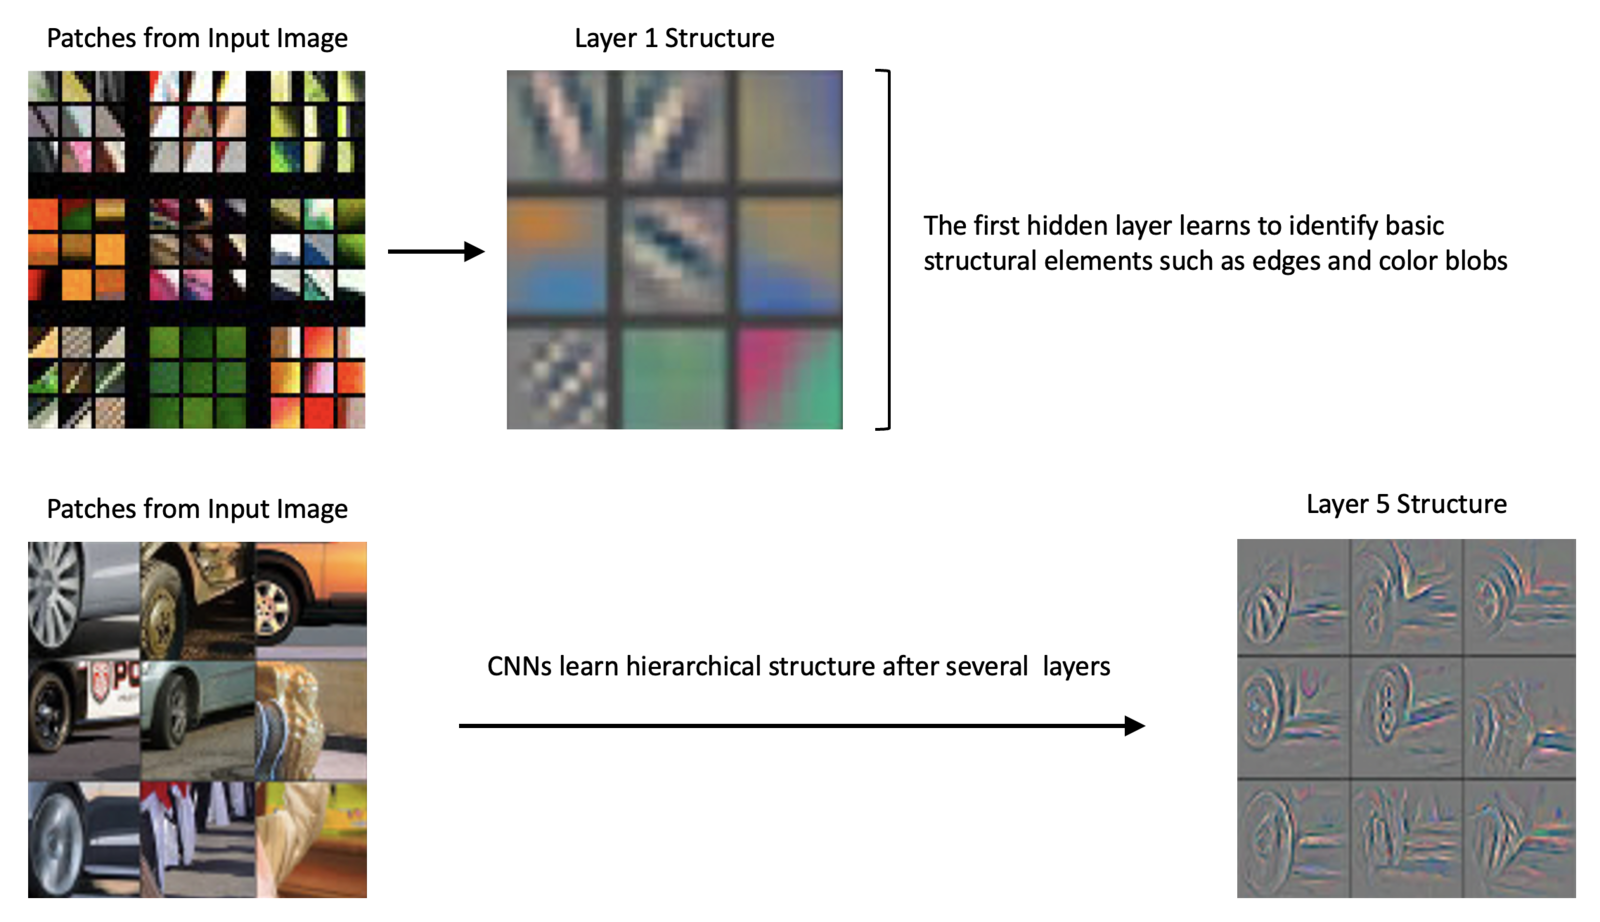
\includegraphics[scale=0.27]{./Images/003_tensorflow-keras-cnn-hierarchical-structure.png}
\caption{Tiefe der Abstraktion von Merkmalen [3]}
\label{Tiefe der Abstraktion von Merkmalen [3]}
\end{figure}

Diese Merkmale sind hierarchisch aufgebaut, das heißt das auf den vorderen Schichten nach simpleren Formen gesucht wird. Auf den späteren Schichten werden diese Merkmale zu komplexen Merkmalen zusammengesetzt.

So wie bei den Pooling Layern, werden in den Convolutional Layern Filter eingesetzt, die über das Inputbild gleiten und eine bestimmte Operation ausführen. Im Gegensatz zu den Pooling Layern, können die Convolutional Layer mehrere Filter besitzen. Dies kann zu großen Mengen an Daten führen, denn jedes Inputbild wird mit jedem Filter verrechnet und sorgt daher für eine weitere Feature Map. Also die Anzahl der Inputbilder, multipliziert mit der Anzahl der Filter, ergibt die Menge der Feature Maps, die an die nächste Schicht weitergegeben werden.
\\
\\
\textbf{Wie Funktioniert die Convolution Operation?}\\
Die Operation besteht aus einer Rechenoperation zwischen den Filtern und der Fläche, über welche sie gelegt werden. Ein Filter besteht aus einer Matrix, welche häufig 3x3 oder 5x5 Felder groß ist. 
Ein Filter wird über das Eingangsbild geschoben, so wie bereits bei den Pooling Layern. Allerdings werden hierbei alle Werte mit den Werten des Filters multipliziert, an den Stellen, an denen sie übereinander liegen. Diese Werte werden addiert und in einer Feature Map gespeichert.
Genau genommen ist diese Operation eine Kreuzkorrelation. Eine Convolution, im Deutschen "Faltung" genannt, wäre eine Kreuzkorrelation, bei der die Filter noch um 180° gedreht werden müssten. Diese Operation kommt aber erst in der Backpropagation vor.
Der Filter kann dabei ganz weit außen starten, oder innerhalb der Grenzen des Eingangsbildes. Wenn der Filter ganz weit außen startet, so dass nur ein einziges Feld mit dem Eingangsbild überlappt, nennt man das eine "Full Cross-Correlation". Wenn der Filter ganz in der oberen linken Ecke startet, dabei aber bereits beim ersten Schritt alle Felder des Filters innerhalb der Grenzen des Eingangsbildes befinden, nennt man das "Valid Cross-Correlation"[7].
In diesem Netzwerk wird die Valid Cross-Correlation verwendet. Die Größe der entstehenden Feature Map hängt ebenfalls davon ab, welche Cross-Correlation verwendet wird. 
Bei der Full Cross-Correlation wird außerhalb der Matrix angefangen. Das bedeutet, dass mehr Schritte benötigt werden, um durch eine Reihe zu iterieren und daher entstehen auch mehr Einträge in der Feature Map.


\begin{figure}[H]
\centering
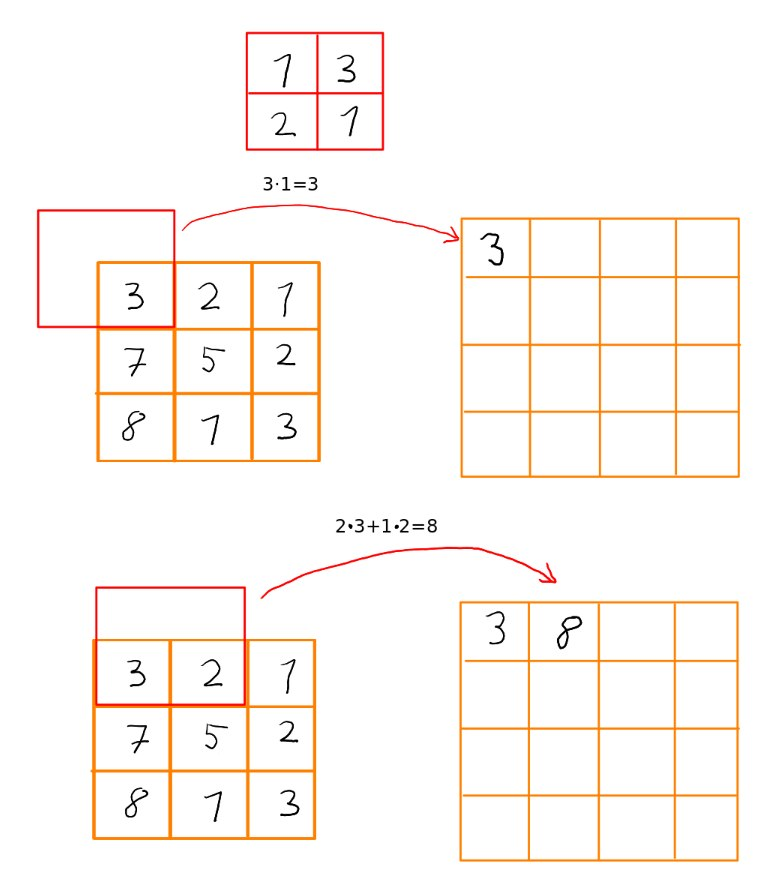
\includegraphics[scale=0.5]{./Images/004_Full_Correlation.jpg}
\caption{Full Cross-Correlation}
\label{Full Cross-Correlation}
\end{figure}
 
Die Valid Cross-Correlation hingegen bewegt sich nur in den Grenzen des Eingangsbildes, daher entstehen weniger Einträge in die Feature Map.


\begin{figure}[H]
\centering
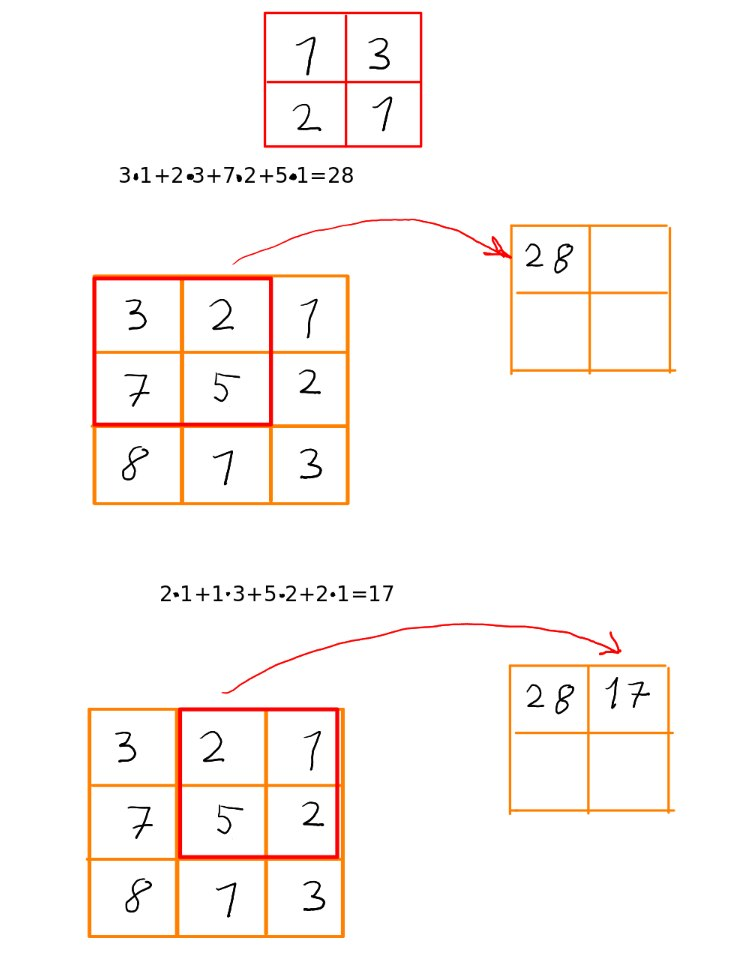
\includegraphics[scale=0.5]{./Images/005_Valid_Correlation.jpg}
\caption{Valid Cross-Correlation}
\label{Valid Cross-Correlation}
\end{figure}

Die Berechnung der Breite und Höhe einer entstehenden Feature Map sind genauso aufgebaut wie zuvor bei den Pool Layern:

$$H_{out} = (H - filter\_height)/stride + 1$$
$$W_{out} = (W - filter\_ width)/stride + 1$$


% TODO Hier müssen mehr erklärungen hin zu der Funktionsweise der Schicht










\cleardoublepage
\subsection{Klassenaufbau der Convolutional Layer}
Grundlegend braucht diese Schicht Filter. Die Filter werden von zwei Parametern gebildet und zwar "filterSize" und "numFilters". Die Größe der Filter wird dabei von "filterSize" festgelegt und "numFilters" beschreibt die Anzahl an Filtern. Wir gehen davon aus, dass die Filter immer quadratisch sind, daher reicht ein Wert um die Größe zu beschreiben.

Darüber hinaus wird wie bei den Pool Layern zuvor, wieder Schrittgrößen, also "stepSize", gebraucht. Diese entscheiden, wie viele Pixel der Filter bei einem Schritt überspringt. Wenn diese größer angelegt werden, werden die Feature Maps dementsprechend kleiner, allerdings kann dies dazu führen, dass Features nicht erkannt und weiterverarbeitet werden. 

Die restlichen Werte die übergeben werden haben mit der Verarbeitung der Eingangs- und Ausgangsbildern zu tun.

Wichtig ist, dass genau wie in den Fully Connected Layern die anpassbaren Werte nicht mit 0 als Startwert initiiert werden, sondern mit zufällig generierten Zahlen. Ansonsten würden die Anpassungen auch immer gleich aussehen. Die Werte, die in dieser Schicht trainiert werden können, sind die Werte in den Filtern.

Hier ist die Constructor Methode der Klasse "ConvolutionLayer":

\begin{lstlisting}[language=Java]
public ConvolutionLayer(int filterSize, int stepSize, int inLength, int inRows, int inCols, int numFilters, double learnRate) {
        this.filterSize = filterSize;
        this.stepSize = stepSize;
        this.inLength = inLength;
        this.inRows = inRows;
        this.inCols = inCols;
        this.learnRate = learnRate;

        generateRandomFilters(numFilters);
    }
\end{lstlisting}

Und in der Methode "generateRandomFilters" werden die Filter generiert und mit Zufallszahlen initiiert. Dabei werden die Filter entsprechend der "filterSize" angelegt und die Liste, welche die Filter enthält ist so groß, wie durch "numFilters" angegeben.

\begin{lstlisting}[language=Java]
private void generateRandomFilters(int numFilters) {
        List<double[][]> filters = new ArrayList<>();
        Random random = new Random();

        for (int n = 0; n < numFilters; n++) {
            double[][] newFilter = new double[filterSize][filterSize];

            for (int i = 0; i < filterSize; i++) {
                for (int j = 0; j < filterSize; j++) {
                    double value = random.nextGaussian();
                    newFilter[i][j] = value;
                }
            }
            filters.add(newFilter);
        }
        this.filters = filters;
    }
\end{lstlisting}

Die entstandenen Filter werden in einer Liste gespeichert. Die Objektvariablen sehen ähnlich wie in den anderen Schichten aus. Die Liste "filters" enthält unsere Filter, inLength entspricht der zusammengefassten Menge aller Inputs aus der vorherigen Schicht. "inRows" und "inCols" beschreiben wieder die Abmaßen der Inputbilder. Auch die Learnrate wird in dieser Schicht, so wie in der Fully Connected Schicht berücksichtigt.

Für die Backpropagation müssen auch hier wieder die Inputs während dem Forwardpass zwischengespeichert werden. Die Liste "lastInput" erfüllt diesen Zweck.

\begin{lstlisting}[language=Java]

public class ConvolutionLayer extends Layer {

    private List<double[][]> filters;
    private int filterSize;
    private int stepSize;

    private int inLength;
    private int inRows;
    private int inCols;
    private double learnRate;

    private List<double[][]> lastInput;

\end{lstlisting}


%\cleardoublepage
\subsection{Forward Propagation im Convolutional Layer}

Die wichtigste Operation im Forwardpass ist die Anwendung der Cross Correlation. Dazu benötigen wir zuerst eine Methode, welche diese Operation auf jedem Inputbild und für jeden Filter anwenden kann. 
Wir erstellen die Methode "convolve". Die Übergabeparameter sind ein Bild, auf dem die Operation angewendet werden soll, ein Filter, der verwendet werden soll und die Schrittweite, wie viele Pixel übersprungen werden sollen:

\begin{lstlisting}[language=Java]
private double[][] convolve(double[][] input, double[][] filter, int stepSize) {
\end{lstlisting}

Als erstes können wir berechnen, wie groß die Feature Map, die entsteht, wird. Die Formel dazu wurde oben bereits erläutert. Die Größe der Filter und die Schrittweite müssen dabei berücksichtigt werden. Die Feature Map kann dann als 2 Dimensionales Array initialisiert werden:

\begin{lstlisting}[language=Java]
int outRows = (input.length - filter.length) / stepSize + 1;
int outCols = (input[0].length - filter[0].length) / stepSize + 1;

double[][] output = new double[outRows][outCols];
\end{lstlisting}

Als nächstes legen wir zur besseren Lesbarkeit zwei Parameter an, welche die Länge und Größe des Inputbildes beinhalten:

\begin{lstlisting}[language=Java]
int inRows = input.length;
int inCols = input[0].length;
\end{lstlisting}

Und wir benötigen auch die Maße des Filters:

\begin{lstlisting}[language=Java]
int fRows = filter.length;
int fCols = filter[0].length;
\end{lstlisting}

Nun müssen wir über das Inputbild iterieren und bei jedem Schritt über den Filter iterieren. Dazu verwenden wir 4 Schleifen. Die äußeren zwei Schleifen wandern über das Bild und die inneren Schleifen wandern über den Filter. 

Um den Überblick zu behalten, an welche Stelle der jeweils berechnete Wert in die Feature Map geschrieben wird, werden die zwei Nummern am Anfang initiiert. Sie enthalten die Koordinate auf der Feature Map, die gerade beschrieben werden soll.

Die ersten zwei Schleifen iterieren über das Inputbild. Der jeweilige Schleifenindex enthält die Koordinate, an welcher der Filter zur Zeit angesetzt werden soll. Dabei soll der Filter von der ersten Reihe oder Zeile, bis zur letzten laufen, allerdings soll der Filter die Grenzen des Bildes nicht überschreiten. Daher wird von der Länge des Bildes, die Länge des Filters abgezogen. Dieser Wert ist der Letzte, bis zu dem der Filter angelegt wird. Der jeweilige Schleifenindex wird bei jeder Iteration um die Schrittlänge erweitert. Auf diese Weise läuft der Filter genau wie gewünscht über das Bild.

Die Feature Map Koordinaten werden Parallel zu den äußeren Schleifen stetig angehoben, allerdings immer nur um eins, da die Feature Map mit jedem Sprung der Filter einen Wert erhält.

\begin{lstlisting}[language=Java]
int featureRow = 0;
int featureCol;
for (int i = 0; i <= inRows - fRows; i += stepSize) {
    featureCol = 0;
    for (int j = 0; j <= inCols - fCols; j += stepSize) {
\end{lstlisting}

Bevor es in die inneren Schleifen geht, muss die Summe initialisiert werden, die später in die Felder der Feature Map eingetragen werden. Die inneren zwei Schleifen iterieren dann über alle Felder des Filters. Um die Position des Feldes auf dem Inputbild zu bestimmen, werden die Werte "inputRowIndex" und "inputColIndex" verwendet, welche lediglich aus der Summe zwischen dem Index der äußeren Zeilen- oder Reihenschleife und der inneren- Zeilen oder Reihenschleife bestehen. Die Position des Filters bestehen aus den Schleifen Indizes. Der Wert aus dem Inputbild und der Wert aus dem Filter werden multipliziert und auf die den "sum" Wert aufaddiert. Sobald alle Felder des Filters abgewandert sind, wird der sum Wert an die entsprechende Stelle in der Feature Map geschrieben.

\begin{lstlisting}[language=Java]
        double sum = 0.0;
        // Hier werden Die Filter Eingesetzt
        for (int x = 0; x < fRows; x++) {
            for (int y = 0; y < fCols; y++) {
                int inputRowIndex = i + x;
                int inputColIndex = j + y;
                double value = filter[x][y] * input[inputRowIndex][inputColIndex];
                sum += value;
            }
        }
        featureMap[featureRow][featureCol] = sum;
        featureCol++;
    }
    featureRow++;
}
return featureMap;  
\end{lstlisting}

Die Feature Map wird dann zurück gegeben. Dies muss allerdings nicht nur für jedes Bild, sondern auch für jeden Filter gemacht werden. Dazu schreiben wir die Methode "convolutionForwardPass". Diese benötigt eine Liste an Inputbildern und gibt eine Liste an Feature Maps zurück:

\begin{lstlisting}[language=Java]
public List<double[][]> convolutionForwardPass(List<double[][]> list) {
    lastInput = list;
    List<double[][]> featureMaps = new ArrayList<>();

    for (int m = 0; m < list.size(); m++) {
        for (double[][] filter : filters) {
            featureMaps.add(convolve(list.get(m), filter, stepSize));
        }
    }
    return featureMaps;
}
\end{lstlisting}

Wichtig hierbei ist zu beachten, dass die Inputbilder in dem Objekt Parameter "lastInput" gespeichert werden. Diese werden für die Backpropagation benötigt.


\subsection{Backpropagation im Convolutional Layer}
Das Konzept der Backpropagation funktioniert im Prinzip so wie zuvor bei den Fully Connected Layern. Jedoch wurden zuvor die Gewichte angepasst, hier, in den Convolutional Layern, werden stattdessen die Filter angepasst. Wie zuvor besprochen, erhofft man sich davon, dass die Filter bestimmte Features erlernen und diese dann erkennen können.
Ebenfalls genau wie zuvor, müssen wir herausfinden, wie viel ein jeder Eintrag im Filter zu dem entstandenen Fehler beigetragen hat. Dazu kann eine Ableitung der ForwardPass Funktion genutzt werden. Anhand der Steigung kann dann abgelesene werden, in welche Richtung die Filter angepasst werden müssen. Dieser Prozess ist aber etwas komplizierter, als in den Fully Connected Schichten. Jeder Eintrag im Filter hat nicht auf alle Felder in einem Inputbild Einfluss. Zum einen wird bei der Valid Cross Correlation nicht jeder Eintrag des Filters über alle Pixel des Bildes gezogen, sondern der Filter bleibt an den Grenzen des Bildes stehen. Und zum anderen wird es noch komplizierter, wenn der Filter eine Schrittgröße über größer als Eins hat. Dann entstehen Lücken, über die der jeweilige Eintrag im Filter springt. All dass muss beachtet werden. 

Wir sehen uns zuerst ein Beispiel für einen Forwardpass an, wobei der Stern Operator hier die Cross-Corelation Operation darstellen soll:
\begin{figure}[H]
\centering
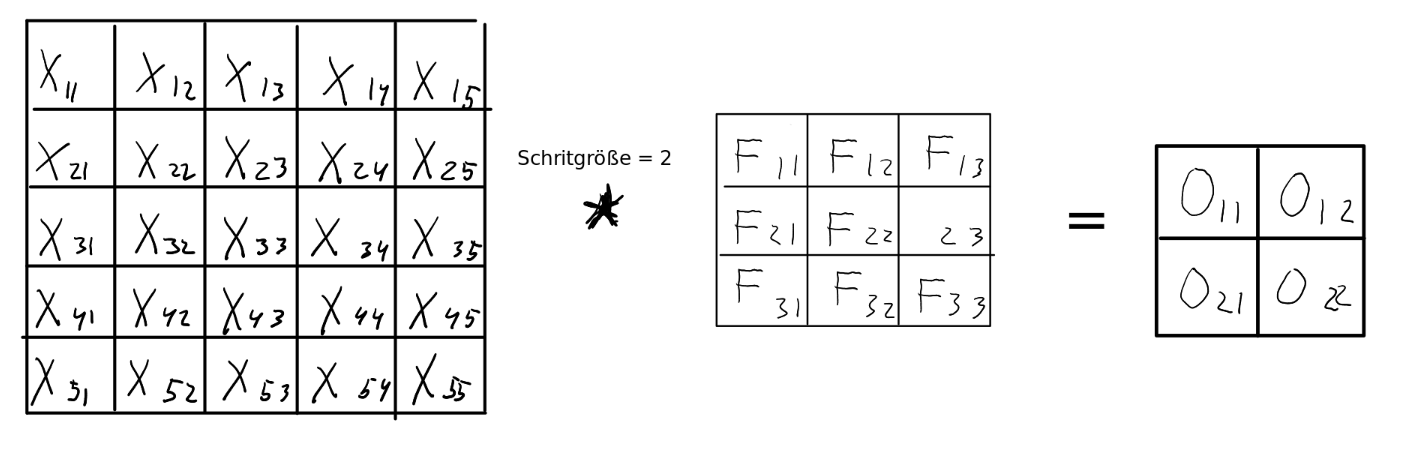
\includegraphics[scale=0.27]{Images/010_ForwardPassConvolution.png}
\caption{Beispiel für Forwardpass}
\label{Beispiel für Forwardpass}
\end{figure}

Das Inputbild hat eine Größe von 5x5 Pixeln, der Filter hat eine Größe von 2x2 und dadurch entsteht ein Output von 2x2, wenn die Schrittgröße 2 Pixel beträgt. 
Wenn nun der Filter auf die erste Stelle gesetzt wird, dann können wir die Rechnung für die Anpassung des ersten Eintrags in der Feature Map anlegen. Anders gesagt, diese Rechnung ist für das Ergebnis in der Feature Map verantwortlich:
$$O_{11} = X_{11}F_{11}+X_{12}F_{12}+X_{13}F_{13}+X_{21}F_{21}+X_{22}F_{22}+X_{23}F_{23}+X_{31}F_{31}+X_{32}F_{32}+X_{33}F_{33}$$
\begin{figure}[H]
\centering
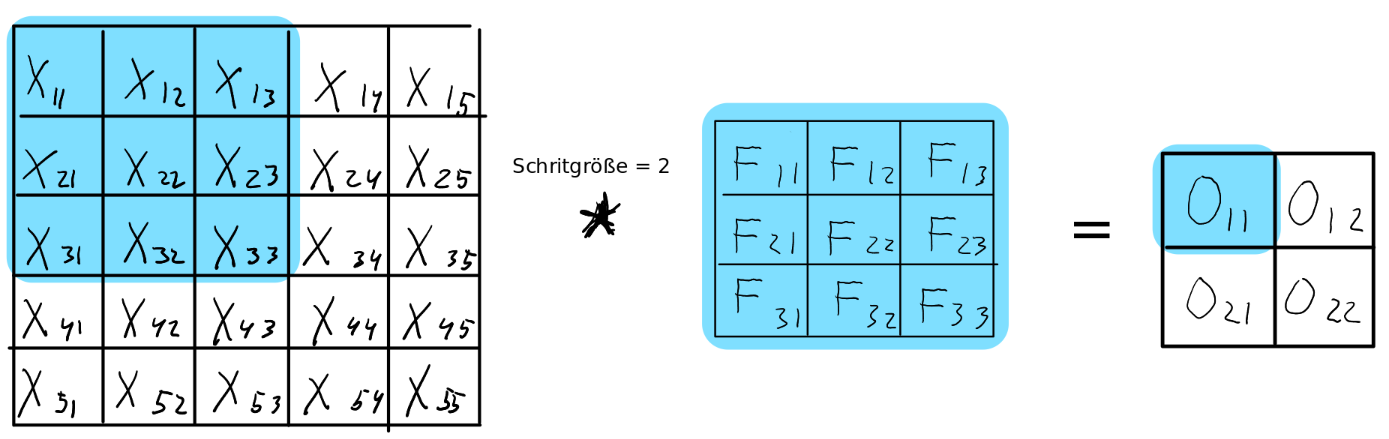
\includegraphics[scale=0.270]{./Images/011_Forward_Pass_ausrechnen_O11.png}
\caption{Forwardpass ausrechnen}
\label{Forwardpass ausrechnen}
\end{figure}

Um nun auszurechnen, wie der Filter angepasst werden sollte, muss die Ableitung der Funktion errechnet werden, im Bezug auf den Eintrag im Filter. Für diese Formel schreiben wir:
$$\frac{dC}{dF_{11}}$$

Wobei $dC$ die Fehlermenge ist, die wir aus der nächsten Schicht oder von der Cost Funktion erhalten und $dF_{11}$ den Eintrag im Filter in erster Reihe und Zeile beschreibt.

Zuerst nutzen wir die Kettenregel um das aufzuschlüsseln. So wie zuvor, wissen wir dass die Costfunction von den Outputs abhängt, die das Netzwerk gibt. Und die Outputs werden direkt von den Filtern beeinflusst. Also haben wir zwei Terme, die Cost Funktion in Abhängigkeit von den Outputs $\frac{dC} {dO} $ und die Outputs in Abhängigkeit zu den Filtern $ \frac{dO} {dF_{11}}$.
$$\frac{dC}{dF_{11}} = \frac{dC} {dO} \frac{dO} {dF_{11}}$$

Allerdings müssen diese weiter aufgeschlüsselt werden. Der Filter hat immerhin Einfluss auf mehrere Outputs, welche wiederum Einfluss auf mehrere Ergebnisse der Cost Funktion haben. Dazu überlegen wir uns einmal, was genau hereingereicht wird. Die Fehler, die zum Beispiel aus einer Fully Connected Schicht hereingereicht werden, entsprechen einer langen Liste mit dem gleichen Format der Inputs, welche jene Schicht erhalten hat. Da wir wissen, auf welche Weise wir die Outputs beim Forwardpass aus mehreren zweidimensionalen Bildern in ein einziges Array sortieren, das heißt die Ausgabe wird "geflattet", können wir diese Formatierung auch rückgängig machen. Solange sich die nächste Schicht an die Konventionen hält, müssten wir in der Lage sein, ein Array an Errors, welches wir von der nächsten Schicht erhalten, in eine Anzahl an Arrays zu formatieren, welche den Maßen der Feature Maps entspricht.
Wir haben dann also eine Reihe an Feature Cost Maps, welche die Abweichungen enthalten, die von den Filtern verursacht wurden. Hier ein Beispiel:

\begin{figure}[H]
\centering
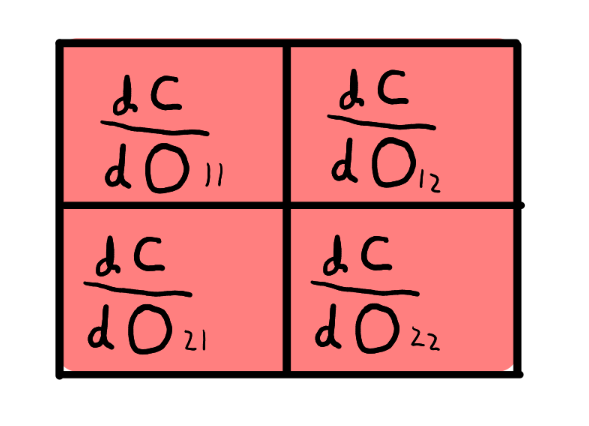
\includegraphics[scale=0.30]{./Images/012_Cost_Deltas.png}
\caption{Cost inputs}
\label{Cost inputs}
\end{figure}

Gehen wir zuerst auf die einzelnen Terme ein. $dC$ ist das Ergebnis der Cost Funktion, so wie zuvor. $dO_{ij}$ entspricht dem Output, der als Eingabe für die Cost Funktion zuständig war.

Mit diesem Filter, der 4 Elemente enthält, entstehen dann also 4 Terme, welche die Formel oben weiter aufschlüsseln:

$$
\frac{dC}{dF_{11}} = 
\frac{dC} {dO} \frac{dO} {dF_{11}}= 
\frac{dC} {dO_{11}} \frac{dO_{11}} {dF_{11}}+
\frac{dC} {dO_{12}} \frac{dO_{12}} {dF_{11}}+
\frac{dC} {dO_{21}} \frac{dO_{21}} {dF_{11}}+
\frac{dC} {dO_{22}} \frac{dO_{22}} {dF_{11}}
$$

$\frac{dO_{11}} {dF_{11}}$ wollen wir zuerst ableiten. Dazu sehen wir uns an, wie die Rechnung der Outputs zu Stande kommt:

$$
O_{11} = X_{11}F_{11}+X_{12}F_{12}+X_{13}F_{13}+X_{21}F_{21}+X_{22}F_{22}+X_{23}F_{23}+X_{31}F_{31}+X_{32}F_{32}+X_{33}F_{33}
$$

Wenn wir nun nach $F_{11}$ ableiten, dann stellt sich heraus, dass nur ein einziger Wert übrig bleibt:

$$\frac{dO_{11}} {dF_{11}} = X_{11}$$

Genau so sieht es mit den anderen Ableitungen der Output Funktion aus, hier noch ein Beispiel:

$$
O_{12} = X_{13}F_{11}+X_{14}F_{12}+X_{15}F_{13}+X_{23}F_{21}+X_{24}F_{22}+X_{25}F_{23}+X_{33}F_{31}+X_{34}F_{32}+X_{35}F_{33}
$$

$$\frac{dO_{12}} {dF_{11}} = X_{13}$$

Die anderen zwei Ableitungen sind:


$$\frac{dO_{21}} {dF_{11}} = X_{31}$$

$$\frac{dO_{22}} {dF_{11}} = X_{33}$$

Wir können das zur besseren Lesbarkeit einmal in die lange Formel von vorhin einsetzten:

%$$
%\frac{dC}{dF_{11}} = 
%\frac{dC} {dO_{11}} X_{11}+
%\frac{dC} {dO_{12}} X_{13}+
%\frac{dC} {dO_{21}} X_{31}+
%\frac{dC} {dO_{22}} X_{33}
%$$

\begin{figure}[H]
\centering
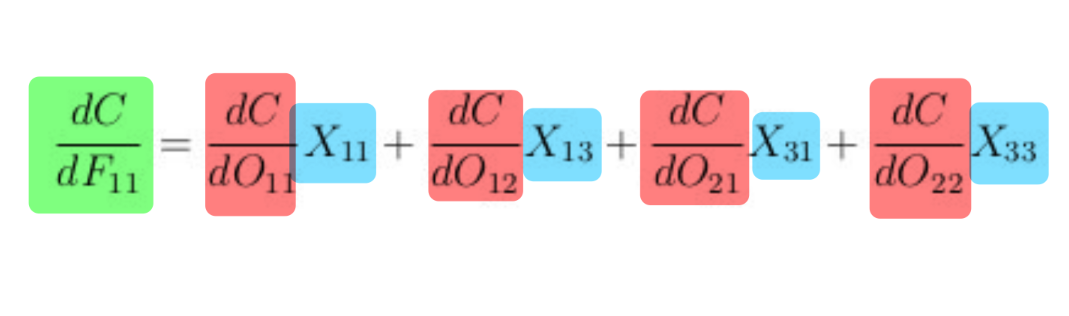
\includegraphics[scale=0.25]{Images/015_BackProp_Delta.png}
\caption{Fehlerrückverfolgung zu einem Filter}
\label{Fehlerrückverfolgung zu einem Filter v1}
\end{figure}

Und einmal mit einer Grafik:
\begin{figure}[H]
\centering
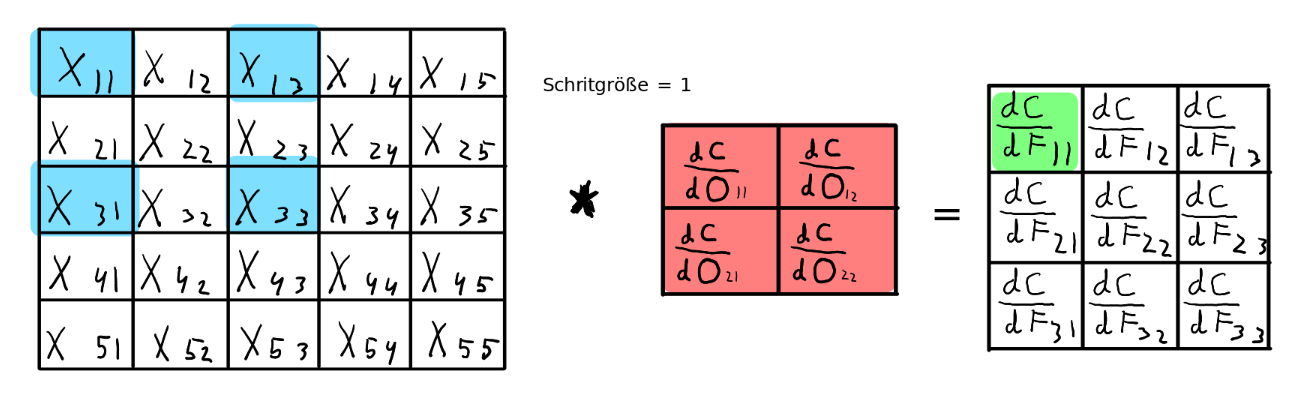
\includegraphics[scale=0.30]{./Images/013_Backpropagation_Filter.png}
\caption{Fehlerrückverfolgung zu einem Filter}
\label{Fehlerrückverfolgung zu einem Filter v1}
\end{figure}

Das die einzelnen Werte auf dem Inputbild jeweils einen Schritt auseinander liegen, liegt daran, dass die Schrittgröße in diesem Beispiel bei 2 liegt. Dadurch wird jeweils ein Pixel übersprungen. Hätten wir hier eine Schrittgröße von 1, dann lägen die Werte beieinander. Oder wenn die Schrittgröße weiter wäre, z.B. bei 3 oder mehr, dann lägen 2 oder mehr Pixel dazwischen.

Die zweite Änderungsrate die wir berechnen wollen, ist $\frac{dC}{dF_{12}}$. 


%$$
%\frac{dC}{dF_{12}} = 
%\frac{dC} {dO_{11}} X_{12}+
%\frac{dC} {dO_{12}} X_{14}+
%\frac{dC} {dO_{21}} X_{32}+
%\frac{dC} {dO_{22}} X_{34}
%$$

\begin{figure}[htp]
\centering
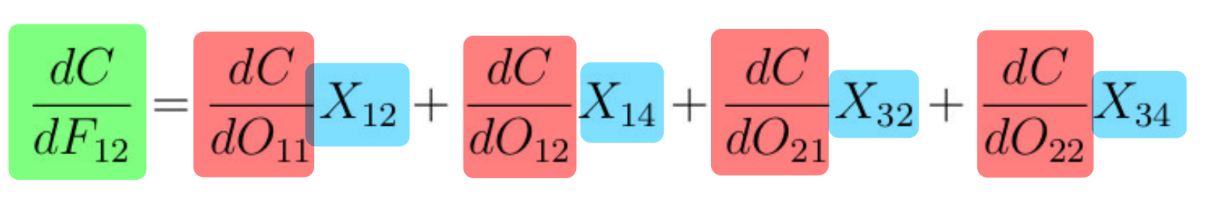
\includegraphics[scale=0.20]{Images/016_BackProp_Delta.png}
\caption{Fehlerrückverfolgung zu einem Filter}
\label{Fehlerrückverfolgung zu einem Filter v2}
\end{figure}

\begin{figure}[H]
\centering
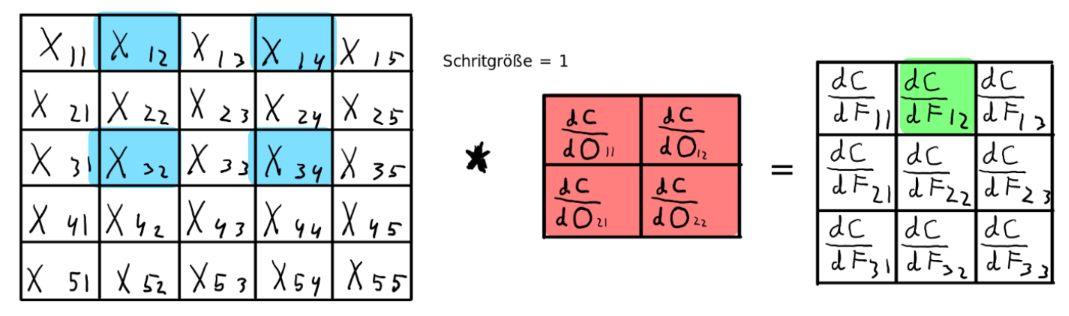
\includegraphics[scale=0.35]{./Images/014_Backpropagation_Filter.png}
\caption{Fehlerrückverfolgung zu einem Filter}
\label{Fehlerrückverfolgung zu einem Filter v2}
\end{figure}

Auch hier wird wieder der Abstand zwischen den Werten eingehalten. Dieses Muster kann für das Netzwerk genutzt werden. 

Das Konzept sieht folgendermaßen aus: Wir erstellen ein Hilfs-Array, welches die Form eines Filters hat und die Fehler, also die Werte $\frac{dC} {dO}$ so angeordnet enthält, dass sie an der richtigen Stelle mit den Werten des Inputbildes verrechnet werden, wenn wir die Convolution Methode anwenden. Auf diese Weise stellen wir sicher, dass für den jeweiligen Eintrag im Filter, der für die Fehler verantwortlich war, genau die Werte im Inputbild verwendet werden, mit denen er auch wirklich zu tun hatte.

Diese Methode nennen wir jetzt "spaceArray". Sie erhält unsere Fehlermatrix und wandelt diese mithilfe der in der Schicht gespeicherten "stepSize" in eine Array um, das wir oben beschrieben haben.

%TODO Es kann noch eine Entscheidung getroffen werden, ob dieser Code Tiefer erklärt werden soll
\begin{lstlisting}[language=Java]
    public double[][] spaceArray(double[][] input) {
        if (stepSize == 1) {
            return input;
        }

        int outRows = (input.length - 1) * stepSize + 1;
        int outCols = (input[0].length - 1) * stepSize + 1;

        double[][] output = new double[outRows][outCols];
        for (int i = 0; i < input.length; i++) {
            for (int j = 0; j < input[0].length; j++) {
                output[i * stepSize][j * stepSize] = input[i][j];
            }
        }
        return output;
    }
\end{lstlisting}

Wenn die Convolution mit dem Hilfsarray abgeschlossen ist, erhalten wir ein Array welches die Änderungsraten enthält, die wir von den Werten im bisherigen Filter abziehen müssen.
Aber danach müssen wir noch die Werte berechnen, die wir an die nächste Schicht im Backpropagationverfahren geben. Genau wie zuvor bei den Fully Connected Layern, leiten wir dann nicht mehr nach den Gewichten, oder hier eben den Filtern ab, sondern nach den Werten in den Inputbildern. Dadurch entsteht wieder eine Ableitung, nämlich $\frac {dC} {dX}$, wobei $X$ die Outputs der vorherigen Schicht repräsentiert, also die Inputbilder der aktuellen Schicht.

Zur Veranschaulichung für unser Beispiel, hier noch einmal die vier Formeln zur Berechnung der Feature Map unseres Beispiels:
$$O_{11} = X_{11}F_{11}+X_{12}F_{12}+X_{13}F_{13}+X_{21}F_{21}+X_{22}F_{22}+X_{23}F_{23}+X_{31}F_{31}+X_{32}F_{32}+X_{33}F_{33}$$
$$O_{12} = X_{13}F_{11}+X_{14}F_{12}+X_{15}F_{13}+X_{23}F_{21}+X_{24}F_{22}+X_{25}F_{23}+X_{33}F_{31}+X_{34}F_{32}+X_{35}F_{33}$$
$$O_{21} = X_{31}F_{11}+X_{32}F_{12}+X_{33}F_{13}+X_{41}F_{21}+X_{42}F_{22}+X_{43}F_{23}+X_{51}F_{31}+X_{52}F_{32}+X_{53}F_{33}$$
$$O_{22} = X_{33}F_{11}+X_{34}F_{12}+X_{35}F_{13}+X_{43}F_{21}+X_{44}F_{22}+X_{45}F_{23}+X_{53}F_{31}+X_{54}F_{32}+X_{55}F_{33}$$

Ziel ist es, herauszufinden, welchen Einfluss die Outputs der vorherigen Schicht auf die Cost Funktion hatte.
Wir sehen uns ein paar Beispiele an. Wenn wir den ersten Wert des Bildes betrachten, war nur der erste Wert im Filter daran beteiligt, den Output zu errechnen. So wird die Kettenregel angewendet:

$$\frac {dC} {dX_{11}} = 
\frac {dC}{dO_{11}} \frac {dO}{dX_{11}} =
\frac {dC}{dO_{11}} F_{11}$$
Um das ein wenig verständlicher darzustellen, visualisieren wir das farblich:
%TODO Bild einfügen für den Oben genannten Umstand

\begin{figure}[H]
\centering
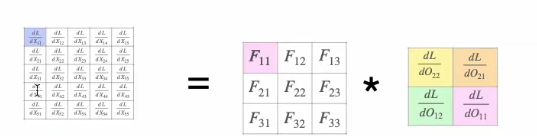
\includegraphics[scale=0.80]{Images/TemporaryPlaceholders/Farbliche Visualisierung der Fehlerrückführung über die Inputs X11.png}
\caption{Farbliche Visualisierung der Fehlerrückführung über die Inputs X11}
\label{Farbliche Visualisierung der Fehlerrückführung über die Inputs X11}
\end{figure}

Nur beim ersten Schritt, wenn der Filter ganz oben in der linken Ecke des Bildes ist, wird der Input $X_{11}$ verwendet. Auch bei $X_{12}$ gibt es nur ein Vorkommen in den Rechnungen:

$$\frac {dC} {dX_{12}} = \frac {dC}{dO_{11}} F_{12}$$

%TODO Ersetze das Bild Dringend
\begin{figure}[H]
\centering
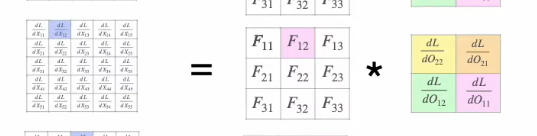
\includegraphics[scale=0.80]{Images/TemporaryPlaceholders/Farbliche Visualisierung der Fehlerrückführung über die Inputs X12.png}
\caption{Farbliche Visualisierung der Fehlerrückführung über die Inputs X12}
\label{Farbliche Visualisierung der Fehlerrückführung über die Inputs X12}
\end{figure}

Anders sieht es allerdings z.B. bei $X_{31}$ aus. Dieser Wert wird sowohl durch den ersten Schritt verwendet, als auch durch den vierten. Das spiegelt sich in der Ableitung wieder:
$$\frac {dC} {dX_{31}} = \frac {dC}{dO_{11}} F_{31} + \frac {dC}{dO_{21}} F_{11}$$

%TODO Ersetze das Bild Dringend
\begin{figure}[H]
\centering
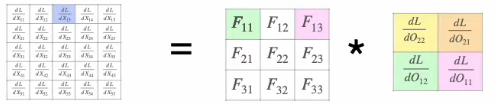
\includegraphics[scale=0.80]{Images/TemporaryPlaceholders/Farbliche Visualisierung der Fehlerrückführung über die Inputs X31.png}
\caption{Farbliche Visualisierung der Fehlerrückführung über die Inputs X31}
\label{Farbliche Visualisierung der Fehlerrückführung über die Inputs X31}
\end{figure}

Hier wird schon sichtbar, dass die Error Map horizontal und vertikal verdreht verwendet wird, aber das wird noch sichtbarer, wenn wir uns $X_{33}$ ansehen. Dieser Wert kommt in allen vier Schritten vor:

$$\frac {dC} {dX_{33}} = \frac {dC}{dO_{11}} F_{33} + \frac {dC}{dO_{31}} F_{11} + \frac {dC}{dO_{21}} F_{13} + \frac {dC}{dO_{22}} F_{11}$$

%TODO Ersetze das Bild Dringend
\begin{figure}[H]
\centering
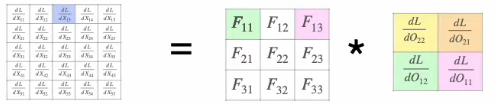
\includegraphics[scale=0.80]{Images/TemporaryPlaceholders/Farbliche Visualisierung der Fehlerrückführung über die Inputs X31.png}
\caption{Farbliche Visualisierung der Fehlerrückführung über die Inputs X33}
\label{Farbliche Visualisierung der Fehlerrückführung über die Inputs X33}
\end{figure}

Wenn man diese Schritte so weiterführen würde, dann werden einem die folgenden Umstände auffallen:
\begin{itemize}
  \item Die Error Map wird vertikal und horizontal gespiegelt verwendet
  \item Die Error Map wird so wie zuvor auch, entsprechend der Schrittgröße auseinander gezerrt  
  \item Bei der oben "Verwendung" genannten Operation handelt es sich um eine Full Cross Correlation
\end{itemize}

Diese Operation kann also auch relativ einfach umgesetzt werden. Wenn wir eine Full Cross-Correlation zwischen der Fehler Map und den bisherigen Filtern ausführen, dann entsteht tatsächlich ein Array, welches die Maße der Inputbilder hat. Dieses Array enthält die Fehlermengen für die nächste Schicht im Backpropagationverfahren. 

Fangen wir doch mit der Full Cross-Correlation an. Die Methode "fullConvolve" erhält die aktuellen Filter und die umgekehrte Error Map als Input. Im Großen und Ganzen können wir die Convolve Methode kopieren, allerdings müssen einige Änderungen vorgenommen werden.

\begin{lstlisting}[language=Java]
private double[][] fullConvolve(double[][] currentFilter, double[][] flippedError) {
        int outRows = (currentFilter.length + flippedError.length) + 1;
        int outCols = (currentFilter[0].length + flippedError[0].length) + 1;
\end{lstlisting}
Zuerst müssen die Outputs anders berechnet werden. Bei der Full Cross-Correlation entstehen mehr berechnete Werte. 
$$H_{out} = (H + filter\_height)-1$$
$$W_{out} = (W + filter\_ width)-1$$
Jedoch kommt es leider immer wieder vor, dass durch die Rundungen beim berechnen der Output Dimensionen nicht ganz die gleichen Matrizen entstehen, wie sie erwartet werden. Durch einige Tests konnte sichergestellt werden, dass eventuelle Überhänge keine notwendigen Informationen enthalten. Allerdings muss man hier aufpassen, dass die "add" Methode, welche die Werte von zwei Arrays addiert, nur über das kleinere Array iteriert. Diese Stellen im Code funktionieren soweit, in zukünftigen Anpassungen können sie aber verbessert werden. Dazu mehr im Abschluss Kapitel, unter möglichen Verbesserungen.

Als nächstes werden die Dimensionen des Filters gespeichert. Über diesen Filter wird wie über das Inputbild iteriert, daher benötigen wir die Abmaßen. Danach nehmen wir die Dimensionen der umgekehrten und auseinander gezerrten Error Map. Diese werden nicht nur für die Iteration in den inneren Schleifen benötigt, sondern diesmal auch für die Begrenzung in den äußeren Schleifen. 
\begin{lstlisting}[language=Java]
        int inRows = currentFilter.length;
        int inCols = currentFilter[0].length;

        int fRows = flippedError.length;
        int fCols = flippedError[0].length;

        double[][] output = new double[outRows][outCols];
        
\end{lstlisting}
        Da es sich hierbei um eine Full Cross-Correlation handelt, wird die erste Position, an welcher der Filter angelegt wird, außerhalb des Inputbildes sein. Das Reflektieren wir dadurch, dass die Startposition in der Schleife die negative Länge der Filters plus eins ist. Dadurch ist nur der äußerste Wert i, Filter über dem ersten Wert im Inputbild.
\begin{lstlisting}[language=Java]

        int outRow = 0;
        int outCol;

        for (int i = -fRows +1; i < inRows; i++) {
            outCol = 0;
            for (int j = -fCols +1; j < inCols; j++) {

                double sum = 0.0;

\end{lstlisting}
Vor den inneren Schleifen, welche über alle Felder des Filters iterieren, initiieren wir die "sum", welchem die einzelnen Berechnungen über allen Einträgen des Filters aufaddiert werden. Die inneren Schleifen funktionieren genau wie zuvor auch, mit dem einzigen Unterschied, dass wir einen Test einbauen müssen, der überprüft, ob ein Wert, der unter einem Filtereintrag außerhalb der Input Matrix liegt. Dadurch vermeiden wir "Index out of Bound Errors".
\begin{lstlisting}[language=Java]
                for (int x = 0; x < fRows; x++) {
                    for (int y = 0; y < fCols; y++) {
                        int inputRowIndex = i + x;
                        int inputColIndex = j + y;

                        if (inputRowIndex >= 0 && inputColIndex >= 0 && inputRowIndex < inRows
                                && inputColIndex < inCols) {
                            double value = flippedError[x][y] * currentFilter[inputRowIndex][inputColIndex];
                            sum += value;
                        }
                    }
                }
                
\end{lstlisting}
Zuletzt werden die Ergebnisse in dem Outputarray gespeichert. Es kann vorkommen, dass dieses Größer ist, als die Abmaße der Inputbilder, allerdings sollte das kein Problem sein. 
\begin{lstlisting}[language=Java]
                output[outRow][outCol] = sum;
                outCol++;
            }
            outRow++;
        }
        return output;
    }
\end{lstlisting}

Kommen wir nun zum Kern, dem eigentlichen "backPropagation" Algorithmus. Wie oben besprochen, benötigen wir eine Liste "filtersDelta" mit den Filter, welche die Änderungsraten für die aktuellen Filter enthalten und eine Liste mit den Ableitungen der Cost Funktion im Bezug auf die aktuellen Filter, "dLd0PreviousLayer", welche wir an die vorherige Schicht weiterleiten werden.
Die "filtersDelta" Liste sollte so initialisiert werden, dass sie genau der Liste mit den Filtern entspricht, das heißt die gleiche Anzahl an Matrizen und diese in gleicher Form und Größe wie die Filter.

\begin{lstlisting}[language=Java]
public void backPropagation(List<double[][]> dLdO) {
        List<double[][]> filtersDelta = new ArrayList<>();
        List<double[][]> dLd0PreviousLayer = new ArrayList<>();;
        for (int f = 0; f < filters.size(); f++) {
            filtersDelta.add(new double[filterSize][filterSize]);
        }
\end{lstlisting}
Nun iterieren wir über alle Inputbilder, die bei dem Forwardpass zwischengespeichert wurden. Wir initialisieren eine Matrix, "errorForInput", um die Fehler für die nächste Schicht aufaddieren zu können.
\begin{lstlisting}[language=Java]
        for (int i = 0; i < lastInput.size(); i++) {
            double[][] errorForInput = new double[inRows][inCols];
\end{lstlisting}
Und dann iterieren wir für jeden Filter, den wir haben und berechnen die Werte, so wie oben beschrieben.
Zuerst speichern wir den aktuellen Filter zwischen, damit wir ihn nachher unverändert verwenden können. Dann holen wir uns die aktuelle Error Map und speichern diese auch.
\begin{lstlisting}[language=Java]
            for (int f = 0; f < filters.size(); f++) {
                double[][] currentFilter = filters.get(f);
                double[][] error = dLdO.get(i * filters.size() + f);
\end{lstlisting}
Der Error muss entsprechend der Schrittgröße auseinandergezogen werden und kann dann an die "convolve" Methode übergeben werden. Die Schrittgröße, die an die Methode übergeben wird, ist hier immer eins, da wir bereits durch das Strecken der Error Map dafür sorgen, dass die jeweilige Schrittgröße berücksichtigt wird.
\begin{lstlisting}[language=Java]
                double[][] spacedError = spaceArray(error);
                double[][] dLdF = convolve(lastInput.get(i), spacedError, 1);
\end{lstlisting}
Nachdem wir also die Änderungsraten berechnet haben, müssen wir sie auch abziehen. Dafür verwenden wir die Methode "multiply", welche jeden Wert eines Arrays mit einem übergebenem Wert multipliziert. Dadurch kehren wir die Werte um, wonach sie danach mithilfe der "add" Methode zu den bisherigen Filter Änderungsraten hinzugefügt werden.
\begin{lstlisting}[language=Java]
                double[][] delta = multiply(dLdF, learnRate * -1);
                double[][] newTotalDelta = add(filtersDelta.get(f), delta);
                filtersDelta.set(f, newTotalDelta);
\end{lstlisting}
Zuletzt kehren wir die gezerrte Error Map auf beiden Achsen um, führen dann die Full Cross-Correlation zwischen ihr und dem aktuellen Filter aus, addieren das Ergebnis auf die bisherige "errorForInput" Matrix, die nachher weitergereicht wird. Und damit ist das Ende der inneren Schleife erreicht.
\begin{lstlisting}[language=Java]
                double[][] flippedError = flipArray(spacedError);
                errorForInput = add(errorForInput, fullConvolve(currentFilter, flippedError));
            }
\end{lstlisting}
Die Matrix "errorForInput" wird in die Liste der Werte für die nächste Schicht eingefügt. Das war der letzte Schritt der Schleife. Zum Schluss müssen die Filter mit den Änderungsraten in "filtersDelta" verrechnet werden und falls es eine vorherige Schicht gibt, sollen auch die Error Maps an die nächste Backpropagationmethode weitergereicht werden.
\begin{lstlisting}[language=Java]
            dLd0PreviousLayer.add(errorForInput);
        }
        for (int f = 0; f < filters.size(); f++) {
            double[][] modified = add(filtersDelta.get(f), filters.get(f));
            filters.set(f, modified);
        }
        if(previousLayer != null){
            previousLayer.backPropagation(dLd0PreviousLayer);
        }
    }
\end{lstlisting}

Damit kommen wir zum Schluss dieses Kapitels. Der gesamte Code ist auf GitHub zu finden:
https://github.com/AkumaKater/Bachelorarbeit
https://git.inf.fh-dortmund.de/01/jafor003/Bachelorarbeit
Die nächsten Kapitel behandeln den Code, der die Schichten verwaltet. 

\cleardoublepage
\section{Verwaltung der Schichten}
In diesem Kapitel gehen wir technisch über den Code, der die Schichten zu einem Netzwerk verbindet.
Um die Schichten zu verwalten, verwenden wir eine Klasse, die wir "NeuralNetwork" nennen. Diese Klasse speichert alle Schichten in einer Liste:

\begin{lstlisting}[language=Java]
public class NeuralNetwork {

    List<Layer> Layers;
    double scaleFactor;

    public NeuralNetwork(List<Layer> Layers, double scaleFactor) {
        this.Layers = Layers;
        this.scaleFactor = scaleFactor;
        linkLayers();
    }
\end{lstlisting}
In der Konstruktor Methode wird die Liste mit den Schichten übergeben. Diese erstellen wir mit einer Builder Klasse, darauf wird im folgenden noch eingegangen. Der "Scalefactor", der auch übergeben wird, wird dazu verwendet, alle Werte in den Inputbildern stark zu verkleinern. Dies hilft den Schichten, die Werte besser zu verarbeiten.
Bei einigen Tests stellte sich heraus, dass das Netzwerk ohne den Scale Factor große Schwierigkeiten hatte, die Trainingsdaten zu lernen.

In der Konstruktor Methode wird außerdem die Methode "linkLayers" aufgerufen. Diese iteriert über alle Schichten und belegt in ihnen die Referenzen auf die anliegenden Schichten:
\begin{lstlisting}[language=Java]
    public void linkLayers(){
        if(Layers.size()<=1){
            return;
        }
        for(int i=1;i<(Layers.size()-1);i++){
            Layers.get(i).setNextLayer(Layers.get(i+1));
            Layers.get(i).setPreviousLayer(Layers.get(i-1));
        }
        Layers.get(0).setNextLayer(Layers.get(1));
        Layers.get(Layers.size()-1).setPreviousLayer(Layers.get(Layers.size()-2));
    }
\end{lstlisting}

\subsection{NeuralNetwork}
Das Netzwerk wird durch die "NeuralNetwork" Klasse repräsentiert. Sie enthält die drei wichtigsten Funktionen eines Netzwerks:
\begin{itemize}
  \item Klassifiziern
  \item Trainieren
  \item Testen
\end{itemize}

\subsubsection{Klassifizieren}

Um ein Bild dem Netzwerk zu übergeben, haben wir die Methode "guess". Diese nimmt ein Image Objekt entgegen und übergibt dieses an die erste Schicht im Netzwerk, an die Methode "getOutput". Diese ist wie wir zuvor gesehen haben, rekursiv aufgebaut und reicht das Inputbild verarbeitet an die nächste Schicht weiter, bis die letzte Schicht ein Ergebnis zurückgibt, welches durch alle Schichten hindurch zurück an diese Stelle kommt. Das Ergebnis ist ein Array, in welchem jedes Feld eine Antwortmöglichkeit des Netzwerks repräsentiert und je höher die Zahl auf dem Feld, desto eher klassifiziert das Netzwerk das Bild als die Antwort, die von dem Feld repräsentiert wird.
\begin{lstlisting}[language=Java]
public int guess(Image image){
        List<double[][]> inList = new ArrayList<>();
        inList.add(multiply(image.getData(), (1.0/scaleFactor)));
        double[] out = Layers.get(0).getOutput(inList);
        int guess = getHighestIndex(out);
        
        return guess;
    }
\end{lstlisting}
Der größte Wert kann als die Antwort des Netzwerks Repräsentiert werden, je weiter diese Zahl von den anderen Möglichkeiten entfernt ist, desto eher kann man interpretieren, dass das Netzwerk sich sehr sicher mit der Antwort ist. Wenn mehrere Werte sehr dicht beieinander liegen, kann man dies so interpretieren, dass sich das Netzwerk nicht sicher ist. Auch wie nah das Ergebnis an der 1 ist lässt Rückschlüsse darüber zu, wie überzeugt das Netzwerk davon ist, dass die Antwort richtig sein sollte.

Um den größten Wert zu ermitteln verwenden wir die Methode "getHighestIndex". Diese gibt den Index des Arrays zurück, welche den größten Wert enthält und repräsentiert damit die Antwort des Netzwerkes.
\begin{lstlisting}[language=Java]
    public static int getHighestIndex(double[] numbers) {
        int maxNumberIndex = 0;

        // Schleife durch das Array laufen und die größte Zahl finden
        for (int i = 0; i < numbers.length; i++) {
            if (numbers[i] > numbers[maxNumberIndex]) {
                maxNumberIndex = i;
            }
        }
        if(maxNumberIndex>9){
            System.out.print(maxNumberIndex);
        }
        return maxNumberIndex;
    }
\end{lstlisting}

\subsubsection{Trainieren}

Die wohl wichtigste Funktion eines Netzwerkes ist die Fähigkeit, zu lernen. Dazu benutzen wir die "train" Methode. Diese erhält eine Liste an Image Objekten, welche die Inputbilder und die Label enthalten, welche die Bilder korrekt beschreiben.
\begin{lstlisting}[language=Java]
public void train (List<Image> images){
        int index = 0;
        for(Image img : images){
            List<double[][]> inList = new ArrayList<>();
            inList.add(multiply(img.getData(), (1.0/scaleFactor)));
            double[] out = Layers.get(0).getOutput(inList);
            double dCdO[] = getErrors(out, img.getLabel());

            Layers.get((Layers.size()-1)).backPropagation(dCdO);

            System.out.print("Prozent: "+index*100/images.size()+"%");
            System.out.print('\r');
            index++;
        }
        System.out.println("Prozent: 100%");
    }
\end{lstlisting}
Auch hier werden die Bilder mit dem Scale Factor angepasst und danach wird jedes Bild einzeln durch den Forward Pass der Methoden gegeben, analog zum Vorgang in der "guess" Methode. Das Array, welches dabei entsteht und die Antwort des Netzwerks enthält, wird dann an die Methode "getErrors" übergeben. Diese berechnet uns die Fehlermenge, die wir für den ersten Schritt im Backpropagation Algorithmus benutzen. Dieser wird dann auch auf der letzten Schicht im Netzwerk aufgerufen.

\begin{lstlisting}[language=Java]
private double[] getErrors(double[] networkOutput, int correctAnswer){
        int numClasses = networkOutput.length;
        double[] expected = new double[numClasses];
        expected[correctAnswer] = 1;
        return add(networkOutput, multiply(expected, -1));
    }
\end{lstlisting}

\subsubsection{Testen}

Abschließend sollte es möglich sein, die Effizienz eines Netzwerkes zu testen. Dazu übergeben wir eine Testmenge an Bildern an die Methode "test". Diese iteriert über alle Inputbilder, verwendet die "guess" Methode um das Ergebnis des Netzwerkes mit dem Label des Bildes zu vergleichen und errechnet dann prozentual den Anteil an richtig klassifizierten Bildern.

\begin{lstlisting}[language=Java]
    public float test (List<Image> images){
        int correct = 0;
        for(Image img : images){
            int guess = guess(img);
            if(guess == img.getLabel()){
                correct++;
            }
        }
        return ((float)correct/images.size());
    }
 \end{lstlisting}

\subsection{NetworkBuilder}
Der Network Builder wird dazu verwendet, um Netzwerke nach bestimmten Merkmalen zu erstellen. Es gibt einige Werte, die wir nicht manuell eingeben müssen, weil sie vollständig von den anderen Schichten im Netzwerk abhängen. Mithilfe dieser Klasse muss jeweils nur das Nötigste angegeben werden, um die verschiedenen Schichten zu erstellen.
Die Klasse enthält jeweils die Methoden "addConvolutionLayer", "addMaxPoolLayer" und "addFullyConnectedLayer" um die Schichten zu erstellen. Dabei füllt die Methode in Abhängigkeit der vorherigen Schicht jeweils die nötigen Felder im Konstruktor der einzelnen Schichten aus, die von den Ausgaben der vorherigen Schichten abhängen. Hier ein Beispiel:
\begin{lstlisting}[language=Java]
public void addConvolutionLayer(int numFilters, int filterSize, int stepSize, double learnRate){
        if(Layers.isEmpty()){
            Layers.add(new ConvolutionLayer(filterSize, stepSize, 1, inputRows, inputCols, numFilters, learnRate));
        }else{
            Layer previousLayer = Layers.get(Layers.size()-1);
            Layers.add(new ConvolutionLayer(filterSize, stepSize, previousLayer.getOutputLength(), previousLayer.getOutputRows(), previousLayer.getOutputCols(), numFilters, learnRate));
        }
    }
\end{lstlisting}
Die Convolution Schicht ist entweder die erste Schicht im Netzwerk und erhält daher nur einen Input, nämlich das Bild. Wenn es aber nicht das Erste ist, dann erhält es eine Reihe von zum Beispiel Feature Maps und die genaue Menge, die erwartet wird, kann von der vorherigen Schicht abgefragt werden.

Wenn in der Main Methode alle Schichten festgelegt wurden, wird zuletzt die Methode "build" aufgerufen, welche die Liste an Schichten an den Konstruktor eines neuen "NeuralNetwork" Objekts übergibt und dieses Netzwerk dann zurückgibt.
\begin{lstlisting}[language=Java]
public NeuralNetwork build(){
        nn = new NeuralNetwork(Layers, scaleFactor);
        return nn;
    }
\end{lstlisting}

Nun ist das Netzwerk einsatzbereit und kann verwendet werden, um zum Beispiel den MNIST Datensatz zu lernen.


\cleardoublepage
\section{Evaluation}
\subsection{Test verschiedener Konfigurationen}
In diesem Kapitel werden einige Konfigurationen getestet. Wir Trainieren das Netzwerk mit dem MNIST Datensatz. Dies ist ein Datensatz, der 60.000 Trainingsbilder enthält und 10.000 Testbilder. Die Bilder enthalten handgeschriebene Zahlen, auf einer Bildgröße von 28x28 Pixeln. Es kommen die Zahlen 0-9 vor, daher braucht das Netzwerk 10 Outputs, um die 10 Antwortmöglichkeiten zu reflektieren. Alle Konfigurationen werden über 3 Epochen getestet, wobei eine Epoche einen Trainingsdurchlauf über alle Trainingsdaten beschreibt.

Zunächst einmal testen wir nur die Fully Connected Schichten. Dazu erstellen wir ein Netzwerk mit 3 Fully Connected Schichten, jeweils mit 300, 250 und 10 Knoten.
Die Schicht mit 10 Knoten ist die Output Schicht und kommt daher in jeder Konfiguration vor. 
In vier Testläufen wurden in der ersten Epoche Ergebnisse zwischen 50\% und 60\% Genauigkeit erreicht. Die Genauigkeit errechnet sich durch den Anteil an korrekt klassifizierten Bildern innerhalb der Trainingsdaten, also Daten, welche das Netzwerk nicht im Training gesehen hat. 60\%-75\% Genauigkeit wurden in der zweiten Epoche erreicht und in der letzten Epoche wurde bis zu 77\% erreicht.

Nun wollen wir sehen, ob eine einzige Convolution Schicht mit einer Max Pool Schicht bereits einen Unterschied machen kann. Wir fügen eine Schicht hinzu, die 8 Filter besitzt, welche 5x5 groß sind und eine Schrittgröße von 1 benutzt. Dazu kommt eine Max Pool Schicht mit Schrittgröße 2 und Fenstergröße 3.
Hierbei wurden nach der ersten Epoche schon über 70\% erreicht, teilweise sogar bis zu 77\%. 

Für die nächste Testreihe wollen testen, wie effektiv das Netzwerk bleibt, wenn wir die Fully connected Schichten entfernen. Dadurch, dass die Convolution Schichten zusammenhängende Features erkennen und die Fully Connected Schichten dann nur noch die Features einordnen müssen, könnte es sein, dass wir gute Ergebnisse mit weniger Neuronen erlangen. Denn die Daten, die von den Fully Connected Schichten verarbeitet werden müssen, sind viel weniger geworden, da sie nicht mehr alle Pixel verarbeiten müssen.
Die erste Testreihe, mit einer Fully Connected Schicht von 250 Knoten und einer von 10 Knoten erzeugt sehr gute Ergebnisse: 85\% auf den besten Testreihen und über 80\% im Durchschnitt.
und wenn man alle bis auf die Outputschicht weg lässt, dann erhält man immer noch durchschnittlich 75\% Genauigkeit.

Als nächstes wollen wir sehen, welchen Einfluss größere Filter haben. Wir erstellen eine Convolution Schicht, mit 8 Filtern, jeweils 7x7 Pixel groß, Schrittgröße 2 und einer Max Pool Schicht und einer Outputschicht, 10 Knoten.
Die Genauigkeit belief sich zwischen allen Tests auf 85\% bis 88\%. 
	
Dabei stellt sich die Frage, wie die Ergebnisse ausfallen, wenn die Filter kleiner werden. Wir verwenden die gleiche Konfiguration wie im letzten Test, nur verwenden wir 3x3 Filter.
Hierbei erreichen die Testfälle nur bis zu 50\%. 

Versuchen wir nun die Anzahl an Filtern zu erhöhen. Dies erhöht auch den Rechenaufwand, aber die Ergebnisse dürften besser werden. Aus den vorherigen Testreihen haben wir gesehen, dass die Filtergröße 7 gute Ergebnisse erzielt hat, also setzten wir diese wieder ein.
Wir verwenden eine Convolution Schicht mit 16 Filtern je 7x7 Pixel. Schrittgröße 2, wieder eine Max Pool Schicht und eine Fully Connected Outputschicht. Die Testreihen ergaben durchschnittlich 88\% Genauigkeit. Eine weitere Testreihe mit 64 Filtern ergab knapp über 90\%.

Zuletzt wollen wir testen, ob sich das Netzwerk durch den Einsatz mehrerer Convolution Schichten verbessern lässt. Theoretisch sind die Filter dazu da, um Muster zu erkennen. Diese Muster können auch innerhalb von Feature Maps entstehen. Um ein stark vereinfachtes Beispiel zu nennen, betrachten wir eine Acht. Diese besteht aus zwei Ringen, die übereinander liegen. Wenn die erste Schicht nun die Ringe erkennt, dann könnte die zweite Schicht die Ringe als Features in der Feature Map erkennen und dann wiederum erkennen, dass diese übereinander liegen. In der YOLO Architektur werden bis zu 24 Convolution Schichten hintereinander verwendet[5]. Dazu testen wir eine Konfiguration mit zwei Convolution Schichten. Die Erste hat 16 Filter, die Zweite hat 32 Filter. Diese Zahlen sind nicht zufällig gewählt. Die Abstraktionstiefe steigt mit jeder Schicht. In der ersten Schicht werden vielleicht nur horizontale und vertikale Kanten erkannt, dazu schräge Kanten, vielleicht auch schon leichte Kurven, oder Ecken. In der zweiten Schicht werden diese Features schon zu komplexeren Formen verbunden, wie zum Beispiel Kreise, längere Striche und so weiter.
Daher benutzen wir weniger Filter in der ersten Schicht und erhöhen die Anzahl dann pro Schicht.

Wir verwenden 2 Convolution Schichten, je 8 und 16 Filter, von 7x7 Pixel Größe. Schrittgröße in beiden sei 2. Nach 3 Epochen erreicht das Netzwerk 85\% Genauigkeit. Dieses Ergebnis entspricht nicht unbedingt den Erwartungen. 
Bei 3 Schichten konnte keines der Netzwerke über 30\% erreichen. Ein Netzwerk, das mit 3 Convolution Schichten gestartet wurde, musste nach 3 Tagen Rechenzeit und eine Genauigkeit von 28\% nach der ersten Epoche gestoppt werden.
Eine Hypothese ist, dass zu wenig Filter in der ersten Schicht verwendet werden:
Wir erhöhen die Anzahl auf 16 Filter in der ersten Schicht und 32 Filter in der zweiten, jeweils 5x5 groß, mit Schrittgröße 2. Nach drei Epochen erzielen wir 85\%.

Es ist klar, dass diese Netzwerke funktionieren. Die besten Ergebnisse, die in allen Tests erzielt werden konnten, lagen bei knapp über 90\%. 

\subsection{Bewertung des Netzwerkes}
Die Ergebnisse fallen leider hinter den Ergebnissen aus der Projektarbeit zurück. Es fällt aber auf, dass auch beim reinen Einsatz von Fully Connected Schichten nicht die Genauigkeit des Netzwerkes aus der Projektarbeit erreicht wird. Dies kann viele Gründe haben, aber die Wahrscheinlichsten sind diese drei:
\begin{itemize}
\item 1. In den Testreihen wurden keine unterschiedlichen Learnrates getestet.
\item 2. Es wurden keine Batches implementiert.
\item 3. Es kann Fehler im Code geben
\end{itemize}
Unterschiedliche Learnrates wurden im Rahmen dieser Bachelorarbeit nicht mehr getestet, da die Netzwerke zuweilen sehr lange Rechenzeiten haben. Die größeren Netzwerke haben für alle 3 Epochen bis zu 3 Tagen gebraucht. Daher wäre der (Zeit-)Aufwand zu groß geworden. 

Durch den Einsatz von Batches wurden im Fully Connected Network aus der Projektarbeit große Verbesserungen erzielt. Diese wären auch hier erwartbar gewesen. Dazu mehr im Kapitel zum Ausblick.

Zuletzt kann es Fehler im Code geben. Bei einigen Konfigurationen wurden Errors geworfen, die das Programm zum Absturz gebracht haben. Diese Fehler können immer noch auftreten. Darauf wird das nächste Kapitel eingehen.

Außerdem fällt auf, das entgegen der Erwartungen, große Filter bessere Ergebnisse erzielt haben. In verschiedenen Online Foren wurde in Kommentaren erwähnt, dass mit TensorFlow, dem Neuronalen Netzwerk Framework von Google, kleinere Filter von der Größe 3x3 bessere Ergebnisse erzielen. Dies kann unter anderem an dem Datensatz liegen, der hier verwendet wird. Der MNIST Datensatz enthält keine kleinen Details. Die Feutures, wie zum Beispiel Kurven, Kreise und Striche sind einfache Formen, von geringer Komplexität. Daher entstehen vergleichsweise wenige Fehler beim Einsatz von größeren Filtern. Es ist sogar Vorstellbar, dass diese die Erkennung begünstigen, da ein vollständiges Feature bereits ohne hohe Abstraktionstiefe erkennbar ist. Das Fell eines Tieres zum Beispiel besteht aus viel kleineren Details, als es der Hals einer 9.

\subsection{Bemerkungen zum Entwicklungsprozess}
Während der Entwicklung des Netzwerkes ist ganz besonders eine Sache aufgefallen: Durch die Größe der Filter und Wahl der Schrittgröße, kann es vorkommen, dass eine oder mehrere Zeilen und Spalten am Ende eines Inputbildes unberücksichtigt bleiben. Für die Bildklassifikation ist das normalerweise nicht von Bedeutung, allerdings kommt es dadurch bei der Backpropagation dazu, dass wenn zwei Matrizen, nämlich die Filter Matrix mit der Filter-Änderungsraten Matrix aufaddiert werden sollen, eine größer ist als die andere.
Sehen wir uns das Problem einmal an: Gegeben ist ein Inputbild mit der Maßen 6x6. Die Convolution Operation wird mit einem 3x3 Filter durchgeführt und einer Schrittgröße von 2. Wie groß wird die Feature Map? 
$$(6-3)/2+1 = 2,5$$
Natürlich kann die Feature Map keine halbe Zeile oder Spalte enthalten, diese fällt also weg. Wäre das Inputbild nun 5x5 Pixel groß gewesen, dann hätten wir das selbe Ergebnis bekommen, eine Feature Map von der Größe 2x2.
Auch fällt auf, dass der Filter niemals eine Überschneidung mit der sechsten Zeile und Spalte erfährt. Beim ersten Schritt überspannt der Filter die Spalten eins bis drei, beim zweiten Schritt drei bis fünf. Aber niemals sechs. 
Wenn wir nun darüber nachdenken, was während der Backpropagation passiert, dann fällt auf, dass es hier zu gewissen Fehlern kommen muss. Die "convolve" Methode erzeugt eine Matrix, die eigentlich die gleiche Größe haben sollte, wie die Filter Matrix, jedoch die Größe der entstehenden Matrix von den Inputs abhängt. Wenn also die auseinander gezerrte Error Map verwendet wird, dann wird diese in unserem Beispiel die Größe 3x3 haben. Je nachdem, ob die Inputbilder dann 5x5 oder 6x6 Pixel groß waren, entstehen an dieser Stelle unterschiedlich große Filter-Änderungsraten Matrizen
$$(5-3)/1+1 = 3$$
$$(6-3)/1+1 = 4$$
Und somit kann es dann zu dem Fehler kommen, dass die Filter-Änderungsraten Matrix größer sein kann, als die Filter Matrix selbst. Wenn in der "add" Methode nur über die Filter Map iteriert wird, dann entsteht hierbei kein Fehler. Die Änderungsraten sind an den richtigen Stellen. Nur falls es anders herum ist und über die Filter Änderungsraten Matrix iteriert wird, dann kann es zu einer "Array Index Out Of Bounds Exception" kommen. 

Ein ähnliche Fall kann durch die  "fullConvolve" Methode entstehen. Auch hier muss das nicht repariert werden. Die entstehende Matrix kann ohne weiteres großer sein, als die Fehlermatrix, für die vorherige Schicht, es kommt nur darauf an, dass die Fehler an die richtige Stelle kommen und dies ist dadurch sicher gestellt, dass bei beiden die Iteration auf dem jeweils ersten Feld beginnt und nur über die kleinere Map als Grenzen für die Schleifen iteriert wird.


\section{Abschluss}
Kommen wir nun zum Abschluss dieser Bachelorarbeit. In diesem Kapitel betrachten wir die Möglichkeiten, das Netzwerk noch weiter zu verbessern und blicken einmal zurück auf die Bachelorarbeit in einem Fazit.

\subsection{Ausblick}
Um das Netzwerk weiter zu verbessern, wäre der erste Schritt Batches umzusetzen. In der Projektarbeit wurden diese auch eingesetzt, allerdings würde es hier den Rahmen sprengen. Mit Batches ist gemeint, dass die Bilder nicht einzeln, sondern in "Batches" also Gruppen von festgelegter Größe an das Netzwerk übergeben werden. Anstatt dass die Bilder dann direkt Einfluss auf die Gewichte und die Filter haben, würden die Änderungsraten zwischengespeichert werden und erst dann, nachdem alle Bilder in dem Batch verarbeitet wurden, werden die Änderungsraten auf einen Schlag angewandt. Dies hat zwei große Vorteile: Der erste ist Geschwindigkeit. Da nicht mehr nach jedem Bild alle Filter und Gewichte angepasst werden, spart sich der Rechner ein wenig Zeit. Die Zwischenergebnisse werden ohnehin zwischengespeichert, nur der Scope müsste angepasst werden. Damit gemeint ist, dass anstatt die Zwischenergebnisse nach einer Schleife über alle Gewichte neu zu initialisiert, werden eher weitere Änderungsraten von weiteren Bilder hinzugefügt, bis der Batch durchgenommen wurde. Danach erst werden die akkumulierten Änderungsraten von den Gewichten und Filtern abgezogen.

Der zweite Vorteil ist tatsächlich auch Performance. dadurch, das immer nur ein Bild auf die Gewichte oder Filter einwirkt, wird das Netzwerk mit jeder Iteration ein wenig zu stark zum Fehlerminimum für nur ein einziges Bild verändert. Dadurch, dass wir mithilfe der Batches mehrere Zahlen auf einem unveränderten Netzwerk trainieren, finden wir nachher mithilfe der akkumulierten Änderungsraten einen besseren Kompromiss, in welche Richtung die Gewichte angepasst zu werden, um ein besseres Ergebnis für alle Bilder zu erzielen. 

Wenn die Batches eingerichtet wurden, dann müsste es auch möglich sein, eine Parallelisierung des Codes einzurichten. Grundlegend, werden alle Bilder in einem Batch mit dem gleichen Netzwerk klassifiziert. Das bedeutet, dass die Ausgangssituation für alle Bilder in einem Batch gleich ist. Diese können also parallelisiert werden. Alle Bilder können parallel berechnet werden und die Änderungsraten können danach zusammengefasst werden und von den Gewichten und Filtern abgezogen werden. Dadurch dass mehrere Prozessoren dann nebeneinander laufen, könnten wir das Netzwerk deutlich beschleunigen. Rein theoretisch, kann ein Netzwerk mit einer Batch Größe von 64 ebenso viele Bilder in der Zeit berechnen, die ein anderes Netzwerk ohne Batches und Parallelisierung für nur ein Bild braucht. Dazu müsste man aber Grafikarten benutzen, denn diese sind für so eine Art von Aufgabe gut geeignet. 

Dieses Projekt zielt aber nicht nicht auf Effizienz. Das hier programmierte Netzwerk dient Lehrzwecken, wird aber nicht mit den viel weiterentwickelten Netzwerken mithalten können. Hardwarenahe Programmiersprachen könnten viel bessere Ergebnisse erzielen, als es Java könnte. Hardwarebeschleuniger werden heutzutage auch häufig eingesetzt und um diese optimal zu nutzen, müsste das Programm auch darauf ausgelegt werden.

\subsection{Fazit}
In dieser Bachelorarbeit wurde gezeigt, dass es möglich ist, ein Convolutional Network selbständig zu programmieren. Wir haben uns die Konzepte angesehen, die den einzelnen Schichten zugrunde liegen. Dabei wurde die Modularität der Schichten besonders betrachtet. Das entstandene Netzwerk ist in der Lage, mehrdimensionale Bilder zu verarbeiten. Damit gemeint sind Bilder, die nicht nur in Greyscale vorliegen, so wie der MNIST Datensatz, sondern auch Bilder, welche in 3 Farben Kanälen vorliegen: Rot, Grün und Blau. Das Netzwerk hat ein paar Schwächen, aber es demonstriert, wie Convolutional Netzwerke die früheren Feed Forward Netzwerken verbessern.

In den verschiedenen Kapiteln wurde zuerst dargestellt, wie die Feed Forward Schichten funktionieren. Wir haben gesehen auf welche Weise diese Schicht Daten verarbeitet und wie die Gewichte angepasst werden. Außerdem haben wir gesehen, wie die Werte bereitgestellt werden, die von einer beliebigen Schicht benötigt werden, um wiederum die eigenen Fehler zu korrigieren. Das Konzept der Backpropagation durch das Gradient Descent Verfahren wurde bereits in der zuvor ausgearbeiteten Projektarbeit ausführlich behandelt und hier aufgegriffen.

Danach wurden die Pool Layer vorgestellt, am Beispiel der Max Pool Schicht, welche die Feature Maps verkleinert und besonders starke Features hervorhebt.

Zuletzt wurden die Convolution Schichten behandelt. Diese Schichten benutzen Filter, um bestimmte Formen, die auf Englisch "Features" genannt werden, aus den Bildern zu extrahieren. Diese Filter werden automatisch erlernt, genau so wie die Gewichte in den Fully Connected Layern. Das Netzwerk ist in der Lage, durch Trainingsdaten selbständig Filter zu trainieren, welche besondere Merkmale erkennen. 

Danach haben wir uns den Code angesehen, der die Schichten verwaltet und damit nicht nur in der Lage ist, Netzwerke zu erstellen, sondern auch die Funktionalität zur Verfügung zu stellen, um Netzwerke zu trainieren und sie Bilder klassifizieren zu lassen.

Zum Schluss haben wir das Netzwerk mit verschiedenen Konfigurationen getestet und die Ergebnisse bewertet. Wir konnten feststellen, dass das Netzwerk gute Ergebnisse liefern kann, aber wir konnten auch sehen, dass die Implementation noch verbessert werden kann.

Abschließend lässt sich sagen, dass dieses Projekt eine interessante Erfahrung war. Die künstlichen Intelligenzen erfahren aktuell ein gewisses Maß an Mystifizierung durch die Medien, aber zu verstehen, wie sie wirklich funktionieren hilft zu erkennen, wozu die Netzwerke wirklich in der Lage sind und was reine Spekulation ist.

\includegraphics[scale=0.8]{Eigenständigkeit2024.pdf}
\thispagestyle{empty}

\sloppy
\section{Quellen}
\begin{itemize}
\item 1. B. Lenze, Einführung in die Mathematik neuronaler Netze. Berlin: Logos Verlag; 2009.
\item 2. Alexey Kravets (02.03.2024), "Forward and Backward propagation of Max Pooling Layer in Convolutional Neural Networks", URL: https://towardsdatascience.com/forward-and-backward-propagation-of-pooling-Layers-in-convolutional-neural-networks-11e36d169bec
\item 3. Bill Kromydas (08.03.2024), "Understanding Convolutional Neural Network (CNN): A Complete Guide", URL: https://learnopencv.com/understanding-convolutional-neural-networks-cnn/
\item 4. Jan Philipp Fortowski (11.2023.2023), "Wie programmiert man ein einfaches Neuronales Netzwerk", befindet sich im Quellen Ordner
\item 5. Joseph Redmon, Santosh Divvala, Ross Girshick, Ali Farhadi (09.05.2016), "You Only Look Once:
Unified, Real-Time Object Detection", befindet sich im Quellen Ordner, URL: http://pjreddie.com/yolo/
\item 6. Eva-Rae McLean (19.04.2022), "Convolutional Neural Network from Scratch", URL: https://www.youtube.com/playlist?list=PLpcNcOt2pg8k\_YsrMjSwVdy3GX-rc\_ZgN, URL: https://github.com/evarae/CNN\_Tutorial
\item 7. Omar Aflak (23.05.2021), "Convolutional Neural Network from Scratch | Mathematics \& Python Code", URL: https://www.youtube.com/watch?v=Lakz2MoHy6o


\end{itemize}

\cleardoublepage
\section{Abbildungsverzeichnis}
\listoffigures
\end{document}